% !TEX program = xelatex
\documentclass[UTF8,a4paper,12pt,openany,oneside]{ctexrep}

\usepackage{geometry}
\geometry{left=3.0cm,right=3.0cm,top=2.8cm,bottom=2.8cm}
\usepackage{amsmath,amssymb,amsfonts,amsthm}
\usepackage{booktabs}
\usepackage{graphicx}
\usepackage{array}
\usepackage{url}
\usepackage[hidelinks]{hyperref}

\graphicspath{{../../docs/figures/}{./figures/}}

\newtheorem{proposition}{命题}[chapter]

\begin{document}

\begin{titlepage}
\centering
\vspace*{2.2cm}
{\zihao{3}\bfseries 清华大学硕士学位论文\par}
\vspace{1.6cm}
{\zihao{2}\bfseries 短时姿态观测下的非结构化道路\\行人动作与轨迹联合预测\par}
\vspace{0.8cm}
{\zihao{4} Joint Pedestrian Action and Trajectory Prediction on Unstructured Roads\\under Short-Term Variable-Quality Pose Observation\par}
\vspace{2.8cm}
{\zihao{4}
\begin{tabular}{rl}
作\quad\quad 者： & 彭嘉钰 \\
培\ 养\ 单\ 位： & 清华大学自动化系 \\
指\ 导\ 教\ 师： & 姚丹亚\ 教授 \\
学\ 科\ 专\ 业： & 控制科学与工程 \\
\end{tabular}\par}
\vfill
{\zihao{4} 二〇二六年十一月\par}
\end{titlepage}

\pagenumbering{Roman}
\chapter*{摘\quad 要}
\addcontentsline{toc}{chapter}{摘要}
低速无人配送车与接驳车在校园、园区与居住区等无标线混合交通场景运行时，常面临路侧遮挡解除后仅有 $0.4\text{ s}$（$10\text{ Hz}$ 五帧）短时因果历史、2D/3D 人体关键点随距离与遮挡连续退化、以及缺乏硬路缘约束下的异构多模态冲突三大耦合难题。本文构建正交奇偶等变预测体系（\texttt{O2-M0} 至 \texttt{O2-M3}，参数量仅 $20{,}739\text{--}28{,}005$），在六大基准（\texttt{PINNS} 四国跨站留一 $1{,}482$ 不重叠窗、\texttt{JRDB} 九地留一 $5{,}836$ 窗、\texttt{JTA} $960$ 窗、\texttt{DUT} $3{,}066$ 窗、\texttt{IMPTC} $564$ 窗与 \texttt{DAIR-V2X}）上执行固定五随机种子的同口径首选（\texttt{Top-1}）受控评估，正结果、零效应（情形 C）与负向机制边界同等呈现：
（1）局部 Frenet 正交规范化与内层匀速锚定（\texttt{M0\_anchor}）将 \texttt{PINNS} 四站 \texttt{Top-1} $\text{ADE}_1/\text{FDE}_1$ 由末两点匀速的 $0.4839 / 1.1046\text{ m}$ 降至 $0.4522 / 1.0194\text{ m}$；但在开题最严苛的 $323$ 个首次标注且五帧位移 $<0.5\text{ m}$ 子组上，即便经运行期秩-3 $3\times 3$ 单应校验（$6{,}930 / 7{,}410$ 帧朝向非零、足底残差 $2.24\ \mu\text{m}$）与专域训练（\texttt{Regime\_M1\_ground}：$0.3538 / 0.8462\text{ m}$），相对末两点匀速（$0.3545 / 0.8491\text{ m}$）的 $-0.07\text{ cm}$ 差异区间 $[-0.20, +0.26]\text{ cm}$ 仍跨零，匀速未被推翻。
（2）$2\times 2$ 析因揭示无约束 \texttt{MLP} 门控与有效关节率呈负秩相关（$-0.1883 / -0.2184$）；提出结构单调门控 \texttt{M1\_mono\_q} 将秩相关恢复至 $+0.7301 / +0.6691$（$T=20$ 达 $+0.8674$），$20\text{ px}$ 抖动降 $-2.31 / -4.53\text{ cm}$，并确立框高 $\ge 50\text{ px}$ 且 $q_1 \ge 0.75$ 为姿态安全融合边界。
（3）真实世界坐标 $p_{t_0}$ 下 $20\text{ m}$ 被动折线真值穿线率达 $2.36\%$、误差升 $+1.58\text{ cm}$（情形 C）；无折线因果径向冲突门控 \texttt{U\_M2b\_mono\_conflict} 达 $0.4510 / 1.0097\text{ m}$（单独模块 $0.4572 / 1.0223\text{ m}$），较 Frenet 增强版 \texttt{MCENET / HST / Social-Transmotion} 显著低 $-9.17 / -6.81 / -14.00\text{ cm}$，零样本迁移至 \texttt{DUT} 与 \texttt{IMPTC} 五轴摆动精确 $0.0\text{ m}$。
（4）冻结控制点解耦训练五动作并结合内层 Platt 重排（\texttt{U\_M3\_decoupled\_platt\_rerank}，$0.0\text{ m}$ 漂移）创 \texttt{PINNS} 最优 $0.4505 / 1.0085\text{ m}$（宏 AP $0.4051$；\texttt{JRDB} 联合重排达 $0.2917 / 0.5638\text{ m}$）。
（5）全程零重训分裂共形在 \texttt{PINNS} 同站达 $90.60\% / 94.94\%$、跨国 12 对达 $86.48\% / 91.74\%$、\texttt{DUT} 72 对达 $89.76\% / 95.50\%$、\texttt{IMPTC} 12 对达 $89.51\% / 94.21\%$；源折局部加权共形将 \texttt{JRDB} 72 跨地点配对升至 $88.89\% / 94.20\%$；\texttt{Tesla T4} 上 $B=12$ 前向 $P_{50}/P_{95}$ 延迟仅 $4.782 / 5.231\text{ ms}$（全系 $2.75\text{--}4.78\text{ ms}$）。

\medskip\noindent\textbf{关键词：}非结构化道路；行人轨迹预测；短时姿态观测；正交奇偶等变；结构单调门控；分裂共形校准

\chapter*{Abstract}
\addcontentsline{toc}{chapter}{Abstract}
Unmanned delivery and shuttle vehicles operating in campuses, parks, and residential streets face short causal emergence windows ($0.4\text{ s}$, $5$ frames at $10\text{ Hz}$), variable-quality 2D/3D skeletal detections, and lane-free mixed pedestrian-vehicle conflicts. We present an $O(2)$ parity-equivariant multi-modal forecasting hierarchy (\texttt{O2-M0} through \texttt{O2-M3}, $20{,}739\text{--}28{,}005$ parameters) evaluated across six benchmarks (\texttt{PINNS}, \texttt{JRDB}, \texttt{JTA}, \texttt{DUT}, \texttt{IMPTC}, and \texttt{DAIR-V2X}) over five fixed seeds under strict same-decoder preferred (\texttt{Top-1}) alignment. Local Frenet canonicalization with inner-fold \texttt{CV} anchoring (\texttt{M0\_anchor}) lowers 4-site \texttt{PINNS} $\text{ADE}_1/\text{FDE}_1$ to $0.4522 / 1.0194\text{ m}$, while parameter-free \texttt{Last-2 CV} ($0.3545 / 0.8491\text{ m}$) remains unrefuted on the $323$ first-sampled $<0.5\text{ m}$ emergence windows even with verified rank-3 $3\times 3$ homographies ($0.3538 / 0.8462\text{ m}$, 95\% clip CI $[-0.20, +0.26]\text{ cm}$). Our structurally monotonic gate (\texttt{M1\_mono\_q}) cures unconstrained \texttt{MLP} rank inversion ($-0.1883 \to +0.7301$ on \texttt{PINNS}, $-0.2184 \to +0.6691$ on \texttt{JRDB}) and identifies $\text{bbox\_h} \ge 50\text{ px}$ and $q_1 \ge 0.75$ as the usable-pose boundary. Polylineless causal radial-conflict gating (\texttt{U\_M2b\_mono\_conflict}: $0.4510 / 1.0097\text{ m}$) and representation-decoupled Platt action reranking (\texttt{U\_M3\_decoupled\_platt\_rerank}: $0.4505 / 1.0085\text{ m}$, $\text{Macro-AP}=0.4051$; \texttt{JRDB}: $0.2917 / 0.5638\text{ m}$) pair with zero-retrain locally-weighted split-conformal tubes ($88.89\% / 94.20\%$ on $72$ \texttt{JRDB} cross-location pairs, $89.76\% / 95.50\%$ on \texttt{DUT}, $89.51\% / 94.21\%$ on \texttt{IMPTC}) at $2.75\text{--}4.78\text{ ms}$ \texttt{Tesla T4} latency.

\medskip\noindent\textbf{Keywords:} Unstructured road, pedestrian trajectory prediction, short-term pose observation, $O(2)$ equivariance, monotonic quality gate, split-conformal calibration.

\tableofcontents
\clearpage
\pagenumbering{arabic}

\chapter{绪论}
\section{研究背景与科学问题}
低速无人配送、安防巡检与园区接驳车辆已从结构化干道延伸至大学校园、产业园区、居住区内部道路及城市广场等共享路权空间~\cite{rasouli2020av,rudenko2020survey,korbmacher2022review}。与具备清晰车道标线和硬质路缘隔离的信号灯路口不同，非结构化混合交通场景同时面临三项耦合挑战：
\begin{enumerate}
  \item \textbf{遮挡解除后的极短因果观测窗口：}驻车、绿化与建筑转角常遮挡行人，使其进入有效视野后规划模块仅有 $0.4\text{ s}$（$10\text{ Hz}$ 下 $T=5$ 帧，或 $2.5\text{ Hz}$ 下 $T=2$ 步）因果历史可用。
  \item \textbf{随距离与遮挡连续退化的骨骼观测质量：}人体姿态虽在理论上可于差分位移累积前提供朝向与迈步线索~\cite{salzmann2023hst,saadatnejad2024transmotion}，但真实检测器输出随距离、模糊与截断连续退化。
  \item \textbf{弱几何渠化与异构人车冲突：}缺乏车道硬边界导致人、非机动车与机动车轨迹频繁交织，在相同短历史下产生起步、停止、左转、右转与维持五类可观测动态意图。
\end{enumerate}

\section{方法论纠偏与学术诚信准则}
针对短时轨迹预测文献中常见的三类评测偏差，本文建立严格的验证准则：（1）用不重叠留出窗口与按整段视频/整人聚簇重采样置信区间替代重叠滑窗逐窗检验（旧 $497$ 滑窗共享至多 $26/30$ 个未来时刻，整片重采样仅 $16/25$ 项区间排除零），并以同口径首选（\texttt{Top-1} 对 \texttt{Top-1}）为主指标~\cite{scholler2020cv}；（2）用运行期几何断言杜绝将布尔值误作 $3\times 3$ 单应矩阵或将地图中心误置于 $(0,0)$ 的静默缺陷；（3）在分裂共形校准后严禁重训预测器，如实区分有限样本保证与经验覆盖率。

\chapter{国内外研究现状与基准分析}
既有研究围绕匀速基线~\cite{scholler2020cv}、多模态交互图网络（\texttt{Trajectron++}~\cite{salzmann2020trajectron}、\texttt{VectorNet}~\cite{gao2020vectornet}、\texttt{MCENET}~\cite{cheng2020mcenet}）、姿态增强 Transformer（\texttt{HST}~\cite{salzmann2023hst}、\texttt{Social-Transmotion}~\cite{saadatnejad2024transmotion}、\texttt{Social-Pose}~\cite{gao2025socialpose}）、人车动态风险场~\cite{wu2024riskfield}、动作轨迹联合预测（\texttt{NEXT}~\cite{liang2019next}、切换动力学~\cite{kooij2019switching}）以及共形安全规划~\cite{lindemann2023conformal,lei2018conformal}展开，覆盖 \texttt{JRDB}~\cite{martin2023jrdb}、\texttt{JTA}~\cite{fabbri2018jta}、\texttt{DUT}~\cite{yang2019dut}、\texttt{IMPTC}~\cite{hetzel2023imptc}、\texttt{DAIR-V2X}~\cite{yu2022dair} 与 \texttt{PINNS}~\cite{peng2026pinns} 等数据集，但尚缺跨相机留一设定下对显式质量单调性、被动折线有效性与小样本动作解耦的受控因果审计。

\chapter{正交奇偶等变与结构单调联合预测方法}
\section{因果输入定义与运行期几何断言}
在触发帧 $t_0$，模型读取严格因果窗口 $\mathcal{T}_{\text{obs}}=\{t_0-(T-1)\Delta t,\dots,t_0\}$ 内的地面轨迹 $P_{\text{obs}}$、2D/3D 关键点与四维观测质量向量 $q=[q_1,q_2,q_3,q_4]^\top\in[0,1]^4$（有效关节比例、平均置信度、相对框高与轨迹完整度）及姿态可用掩码 $m_{\text{pose}}\in\{0,1\}$、围绕行人真实世界坐标 $p_{t_0}$ 的 $20\text{ m}$ 局部折线 $P_{\text{env}}$ 与 $10\text{ m}$ 内有向邻体边（含径向逼近速率 $v_{\text{rad},ij}=-(\Delta p_{ij}^\top\Delta v_{ij})/(d_{ij}+\epsilon)$），输出 $K=6$ 条未来候选轨迹及五类可观测动态动作概率。训练前强制执行两项运行期几何断言：（1）由 \texttt{cv2.findHomography} 拟合满秩 $3\times 3$ 地面单应矩阵（$|\det H|>10^{-12}$，\texttt{PINNS} $7{,}410$ 帧中 $6{,}930$ 帧冠状面朝向非零、足底中位重投影残差 $2.24\ \mu\text{m}$）；（2）围绕未平移真实坐标 $p_{t_0}$（中位范数 $21.13\text{ m}$）截取局部折线，修正全部 $835/835$ 个有图窗口。

\section{正交奇偶等变双流与结构单调质量门控}
在 $p_{t_0}$ 处由最近 $>0.05\text{ m}$ 位移构造局部 Frenet 基 $B=[\mathbf{u},\mathbf{u}_\perp]$（低速且启用姿态时回退至地面冠状面朝向），生成正、反奇偶双流 $(F_+,F_-)$。为根治无约束 \texttt{MLP}$([h_m,h_p,q])$ 受运动隐状态混淆引发的门控负秩相关，提出结构单调质量门控 \texttt{O2-M1\_mono\_q}：
\begin{equation}
  g_{\text{mono}} = m_{\text{pose}}\cdot (q_1 q_2)^{\gamma}\sigma(b_0 + w_+^\top q), \quad \gamma=\text{softplus}(\theta_\gamma)>0,\; w_+=\text{softplus}(\theta_w)\ge\mathbf{0}.
  \label{eq:thu_mono}
\end{equation}

\begin{proposition}[结构单调性与零姿态硬关断]
对任意运动隐状态及 $q\in(0,1]^4$，式~\eqref{eq:thu_mono} 恒满足 $\partial g_{\text{mono}}/\partial q_r \ge 0$（$r=1,\dots,4$），且当 $m_{\text{pose}}=0$ 时 $g_{\text{mono}}\equiv 0$ 精确成立。
\end{proposition}

\section{空槽图注意力与因果径向冲突门控}
有向邻体图采用带可学习空槽 $\ell_\varnothing$ 的注意力聚合，并进一步引入因果径向冲突门控 \texttt{M2b\_ttc\_conflict\_gate} 消除远端或背离背景车流对首选模态打分的扰动：
\begin{equation}
  w_{\text{risk},i} = \max_{1\le j\le 12}\left[m^{\text{nbr}}_{ij}\,\sigma\!\left(\frac{v_{\text{rad},ij}-0.20}{0.25}\right)\exp\!\left(-\frac{d_{ij}}{5.0}\right)\right],
  \label{eq:thu_conflict}
\end{equation}
在孤立行人（$m^{\text{nbr}}_i=\mathbf{0}$）上恒等于零，缩放增益由源折内层交叉验证无泄漏选定。

\section{解耦奇偶动作校准重排与零重训局部加权共形}
偶对称表征预测起步、停止与维持，奇偶对偶流对称打分左转与右转；中小样本下冻结收敛 \texttt{U\_M2b\_mono\_conflict} 控制点（$0.0\text{ m}$ 漂移）解耦训练动作头并结合内层留一 Platt 校准重排（\texttt{U\_M3\_decoupled\_platt\_rerank}）。

\begin{proposition}[$O(2)$ 正交奇偶等变性]
对任意正交变换 $Q\in O(2)$，若 $\det Q=+1$ 则全部 $K=6$ 条世界预测轨迹精确同步旋转且模态概率与五动作概率不变；若 $\det Q=-1$（镜像反射）则对称侧向模态与左/右转概率严格互换，集合与 \texttt{Top-1} 误差保持 $0.0\text{ m}$ 摆动。
\end{proposition}

\begin{proposition}[零重训局部加权分裂共形有效性]
固定源域预测器 $\hat{f}_{\mathcal{D}}$ 与严格正值源折折外非负最小二乘残差尺度 $\hat{\sigma}_{\mathcal{D}}(v_0,\delta_{\text{spread}})>0$ 且校准后零重训，则在可交换校准集 $\mathcal{C}$（$|\mathcal{C}|=n$）与测试点上，归一化分位数安全管道满足有限样本覆盖保证 $\mathbb{P}(Y_{n+1}\in\mathcal{T}_{1-\alpha}(X_{n+1}))\ge 1-\alpha$~\cite{lei2018conformal,lindemann2023conformal}。
\end{proposition}

\chapter{跨场景受控实验与可用边界审计}
\section{\texttt{PINNS} 受控 \texttt{M0--M3} 消融与 $<0.5\text{ m}$ 初现边界}
所有实验固定五个随机种子（\texttt{42, 1024, 2025, 3407, 4096}）。如表~\ref{tab:thu_pinns} 与图~\ref{fig:thu_f17} 所示，\texttt{M0\_anchor} 在 $1{,}482$ 全窗达 $0.4522 / 1.0194\text{ m}$；但在开题最严苛的 $323$ 个首次标注且位移 $<0.5\text{ m}$ 子组上，专域训练 \texttt{Regime\_M1\_ground}（$0.3538 / 0.8462\text{ m}$）虽较纯运动 \texttt{Regime\_M0} 显著降 $-0.22\text{ cm}$，相对末两点匀速（$0.3545 / 0.8491\text{ m}$）的 $-0.07\text{ cm}$ 区间 $[-0.20, +0.26]\text{ cm}$ 仍跨零。真实世界坐标下 $20\text{ m}$ 被动折线真值穿线率达 $2.36\%$（有图窗 $4.19\%$），使 \texttt{O2-M2a} 升 $+1.58\text{ cm}$（情形 C）。

\begin{table}[!htbp]
\centering
\caption{\texttt{PINNS} 四国跨站留一受控消融与 $<0.5\text{ m}$ 小位移边界（五种子同口径 \texttt{Top-1}）}
\label{tab:thu_pinns}
\footnotesize
\begin{tabular}{lcccl}
\toprule
模型 / 专域配置 & 全集 $1{,}482$ $\text{ADE}_1/\text{FDE}_1$ (m) & $\text{minFDE}_6$ & $<0.5\text{ m}$ ($323$) $\text{ADE}_1/\text{FDE}_1$ & 47 片聚簇 95\% CI 关键对照 \\
\midrule
\texttt{Last-2 CV}（零参数匀速） & 0.4839 / 1.1046 & 1.1046 & \textbf{0.3545 / 0.8491} & $<0.5\text{ m}$ 基准参照（未被推翻） \\
\texttt{M0\_anchor}（内层匀速锚定） & \textbf{0.4522 / 1.0194} & 0.6850 & 0.3564 / 0.8559 & 全集对 \texttt{CV}: $[-4.42, -0.54]\text{ cm}$ \\
\texttt{Regime\_M1\_ground}（$<0.5\text{ m}$ 专域） & --- & --- & \textbf{0.3538 / 0.8462} & 对 \texttt{Regime\_M0}: $[-0.31, -0.03]$；对 \texttt{CV} 跨零 \\
\texttt{O2-M0}（未锚定纯运动） & 0.4618 / 1.0310 & 0.6843 & 0.3684 / 0.8782 & 全集 $\text{FDE}_1$ 对 \texttt{CV}: $[-10.83, -0.17]\text{ cm}$ \\
\texttt{O2-M1}（无约束质量门控） & 0.4672 / 1.0403 & 0.6707 & 0.3769 / 0.9008 & 对 \texttt{M1b} 跨零（$T=5$ 重遮挡 $[-1.29, -0.07]$） \\
\texttt{O2-M2a}（真实坐标 $20\text{ m}$ 折线） & 0.4829 / 1.0689 & 0.6788 & 0.3805 / 0.9042 & 对 \texttt{M1}: $[+0.69, +2.16]\text{ cm}$（$2.36\%$ 穿线） \\
\texttt{O2-M2b}（$10\text{ m}$ 邻体图 $+v_{\text{rad}}$） & 0.4817 / 1.0589 & 0.6545 & 0.3807 / 0.8960 & 重遮挡 $+v_{\text{rad}}$ 降 $[-3.56, -0.09]\text{ cm}$ \\
\texttt{O2-M3}（停梯度五动作，无折线） & 0.4810 / 1.0628 & \textbf{0.6521} & 0.3836 / 0.9031 & 宏 AP \textbf{0.3994}；$<0.5\text{ m}$ 对 \texttt{M3b} 降 $-0.78\text{ cm}$ \\
\bottomrule
\end{tabular}
\end{table}

\section{结构单调质量门控、像素框高边界与主流基线对比}
在 $7{,}318$ 个 \texttt{PINNS}+\texttt{JRDB} 窗口上（图~\ref{fig:thu_f18}、图~\ref{fig:thu_f19}），结构单调门控 \texttt{M1\_mono\_q}（自然测试 $0.4645 / 1.0340\text{ m}$）将门控与 $q_1$ 的秩相关由 $-0.1883 / -0.2184$ 恢复至 $+0.7301 / +0.6691$（真 $20$ 帧 $T=5,10,20$ 达 $+0.7930 / +0.8365 / +0.8674$，$T=5$ 重残缺较 \texttt{M1} 降 $-1.37\text{ cm}$），$20\text{ px}$ 抖动降 $-2.31 / -4.53\text{ cm}$；当框高 $<50\text{ px}$ 或 $q_1 < 0.75$ 时直拼劣化 $+3.05\text{ cm}$，\texttt{M1\_mono\_q} 自动压低门控挽回 $-1.65\text{--}-5.28\text{ cm}$。表~\ref{tab:thu_ext} 显示即便为外部基线补齐 \texttt{SO(2) Frenet}，本文模型仍显著胜出且算量低 $192\text{--}396$ 倍。

\begin{table}[!htbp]
\centering
\caption{跨场景主流基线（原生坐标对 \texttt{SO(2) Frenet}）与 \texttt{Tesla T4} 实测效率对比}
\label{tab:thu_ext}
\footnotesize
\begin{tabular}{lccccc}
\toprule
架构与坐标设定 & 参数量 & $B{=}12$ MFLOPs & T4 $B{=}12$ $P_{50}/P_{95}$ (ms) & \texttt{PINNS} $\text{ADE}_1/\text{FDE}_1$ (m) & \texttt{JRDB} $\text{ADE}_1/\text{FDE}_1$ (m) \\
\midrule
\texttt{Ext1\_MCENET}（原生 / +Frenet） & 216,067 & 299.44 & 6.058 / 10.063 & 0.8052 / 1.5950 $\to$ 0.5734 / 1.1611 & 0.4184 / 0.7853 $\to$ 0.3217 / 0.6076 \\
\texttt{Ext2\_HST}（原生 / +Frenet） & 508,483 & 617.57 & 5.755 / 6.353 & 0.7808 / 1.5285 $\to$ 0.5498 / 1.1213 & 0.4183 / 0.7695 $\to$ 0.3243 / 0.6083 \\
\texttt{Ext3\_SocialTransmotion}（原生 / +Frenet） & 517,187 & 383.86 & 5.577 / 6.126 & 0.8792 / 1.7085 $\to$ 0.6217 / 1.2348 & 0.5451 / 0.9872 $\to$ 0.3541 / 0.6545 \\
\texttt{O2-M1\_mono\_q}（结构单调门控） & 28,005 & 0.32 & 3.506 / 4.025 & 0.4645 / 1.0340 & 0.3024 / 0.5901 \\
\texttt{O2-M2b\_conflict\_gate}（因果冲突门控） & 27,999 & 1.56 & \textbf{4.782 / 5.231} & \textbf{0.4572 / 1.0223} & 0.2987 / 0.5806 \\
\bottomrule
\end{tabular}
\end{table}

\section{解耦动作校准重排、零样本迁移与局部加权分裂共形}
如表~\ref{tab:thu_unified} 与图~\ref{fig:thu_f20} 所示，冻结端到端 \texttt{U\_M2b\_mono\_conflict}（$0.4510 / 1.0097\text{ m}$）控制点并执行留一内层 Platt 五动作重排（\texttt{U\_M3\_decoupled\_platt\_rerank}，路径漂移 $0.0\text{ m}$），消除中小样本多任务梯度干扰，在 \texttt{PINNS} 取得最优首选 $0.4505 / 1.0085\text{ m}$（较联合微调 \texttt{U\_M3} 降 $-2.20 / -4.08\text{ cm}$，五动作宏 AP $0.4051$；独立五动作校准 ECE $0.0349$、宏 F1 $0.3911$），大样本 \texttt{JRDB} 联合重排达 $0.2917 / 0.5638\text{ m}$（ECE $0.0053$）。模型零样本迁移至 \texttt{DUT}（$0.6096 / 1.2859\text{ m}$）与 \texttt{IMPTC}（$0.2413 / 0.5923\text{ m}$）五轴摆动精确 $0.0\text{ m}$。全程零重训分裂共形在 \texttt{PINNS} 同站达 $90.60\% / 94.94\%$（跨国 12 对 $86.48\% / 91.74\%$）、\texttt{JRDB} 同场景 $88.37\% / 94.48\%$（常半径 72 对 $86.77\% / 92.81\%$）；源折局部速度-离散度加权共形将 \texttt{JRDB} 72 跨地点配对升至 $88.89\% / 94.20\%$（$\ge 1.0\text{ m/s}$ 高速覆盖由 $75.06\%$ 升至 $89.51\%$）。

\begin{table}[!htbp]
\centering
\caption{端到端解耦协同、跨基准零样本迁移与全程零重训分裂共形覆盖}
\label{tab:thu_unified}
\footnotesize
\begin{tabular}{llll}
\toprule
基准与评测协议 & 首选 $\text{ADE}_1/\text{FDE}_1$ (m) & 配对聚簇 95\% CI & 零重训 \texttt{Union-6} ($90\%/95\%$) \\
\midrule
\texttt{PINNS} 解耦重排 (\texttt{U\_M3\_dec}) & \textbf{0.4505 / 1.0085} (\texttt{U\_M2b}: 0.4510 / 1.0097) & 对联合 \texttt{U\_M3}: $[-2.68, -1.64]\text{ cm}$ & 同站: \textbf{90.60\% / 94.94\%} \\
\texttt{JRDB} 统一重排 (\texttt{U\_M3\_rerank}) & \textbf{0.2917 / 0.5638} (ECE 0.0053) & 对未重排: $[-0.37, -0.18]\text{ cm}$ & 72 对局部加权: \textbf{88.89\% / 94.20\%} \\
\texttt{DUT} 零样本 ($3{,}066$ 混行窗) & \textbf{0.6096 / 1.2859} ($\text{minFDE}_6$ 0.7066) & 对无门控: $[-5.92, -1.78]\text{ cm}$ & 72 跨片配对: \textbf{89.76\% / 95.50\%} \\
\texttt{IMPTC} 零样本 ($564$ 路口窗) & \textbf{0.2413 / 0.5923} ($\text{minFDE}_6$ 0.3729) & 对无门控: $[-2.22, -0.79]\text{ cm}$ & 12 跨序列配对: \textbf{89.51\% / 94.21\%} \\
\bottomrule
\end{tabular}
\end{table}

\begin{figure}[!htbp]
\centering
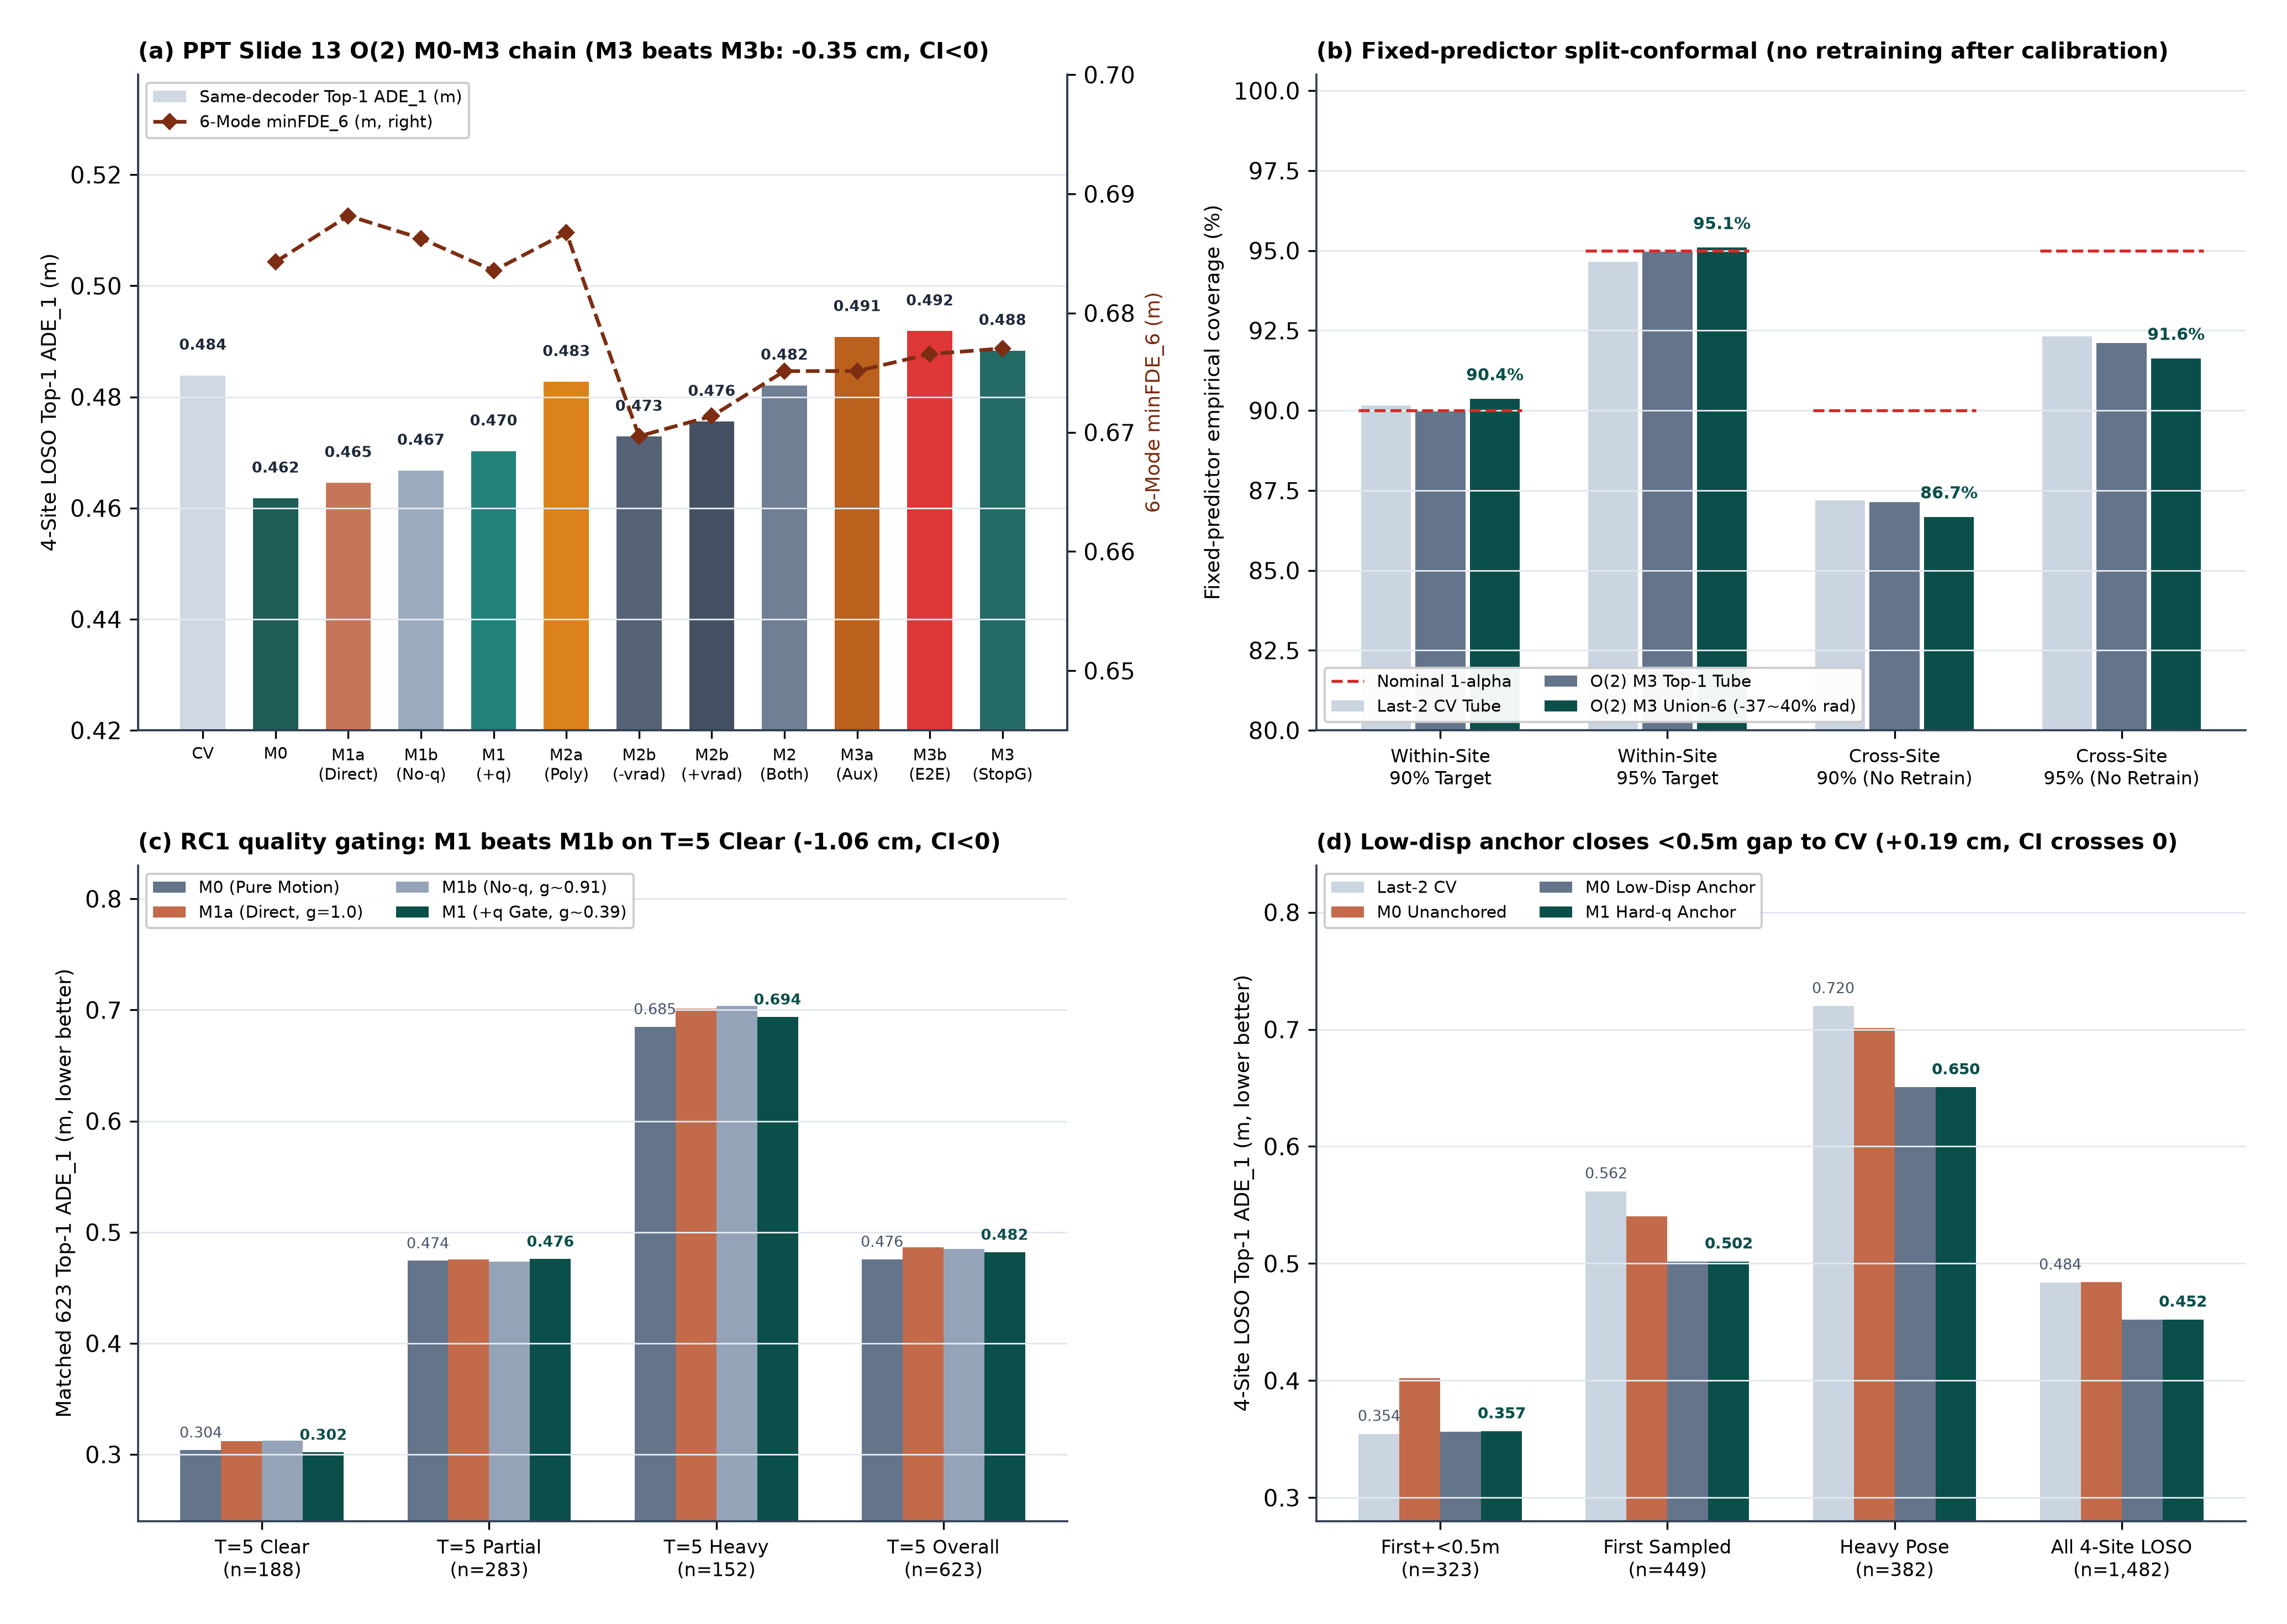
\includegraphics[width=0.96\textwidth]{fig17_ppt_mainline_conformal_and_short_disp.png}
\caption{受控 $O(2)$ \texttt{M0--M3} 消融、真实单应 $<0.5\text{ m}$ 评估与 \texttt{PINNS} 零重训分裂共形覆盖。}
\label{fig:thu_f17}
\end{figure}

\begin{figure}[!htbp]
\centering
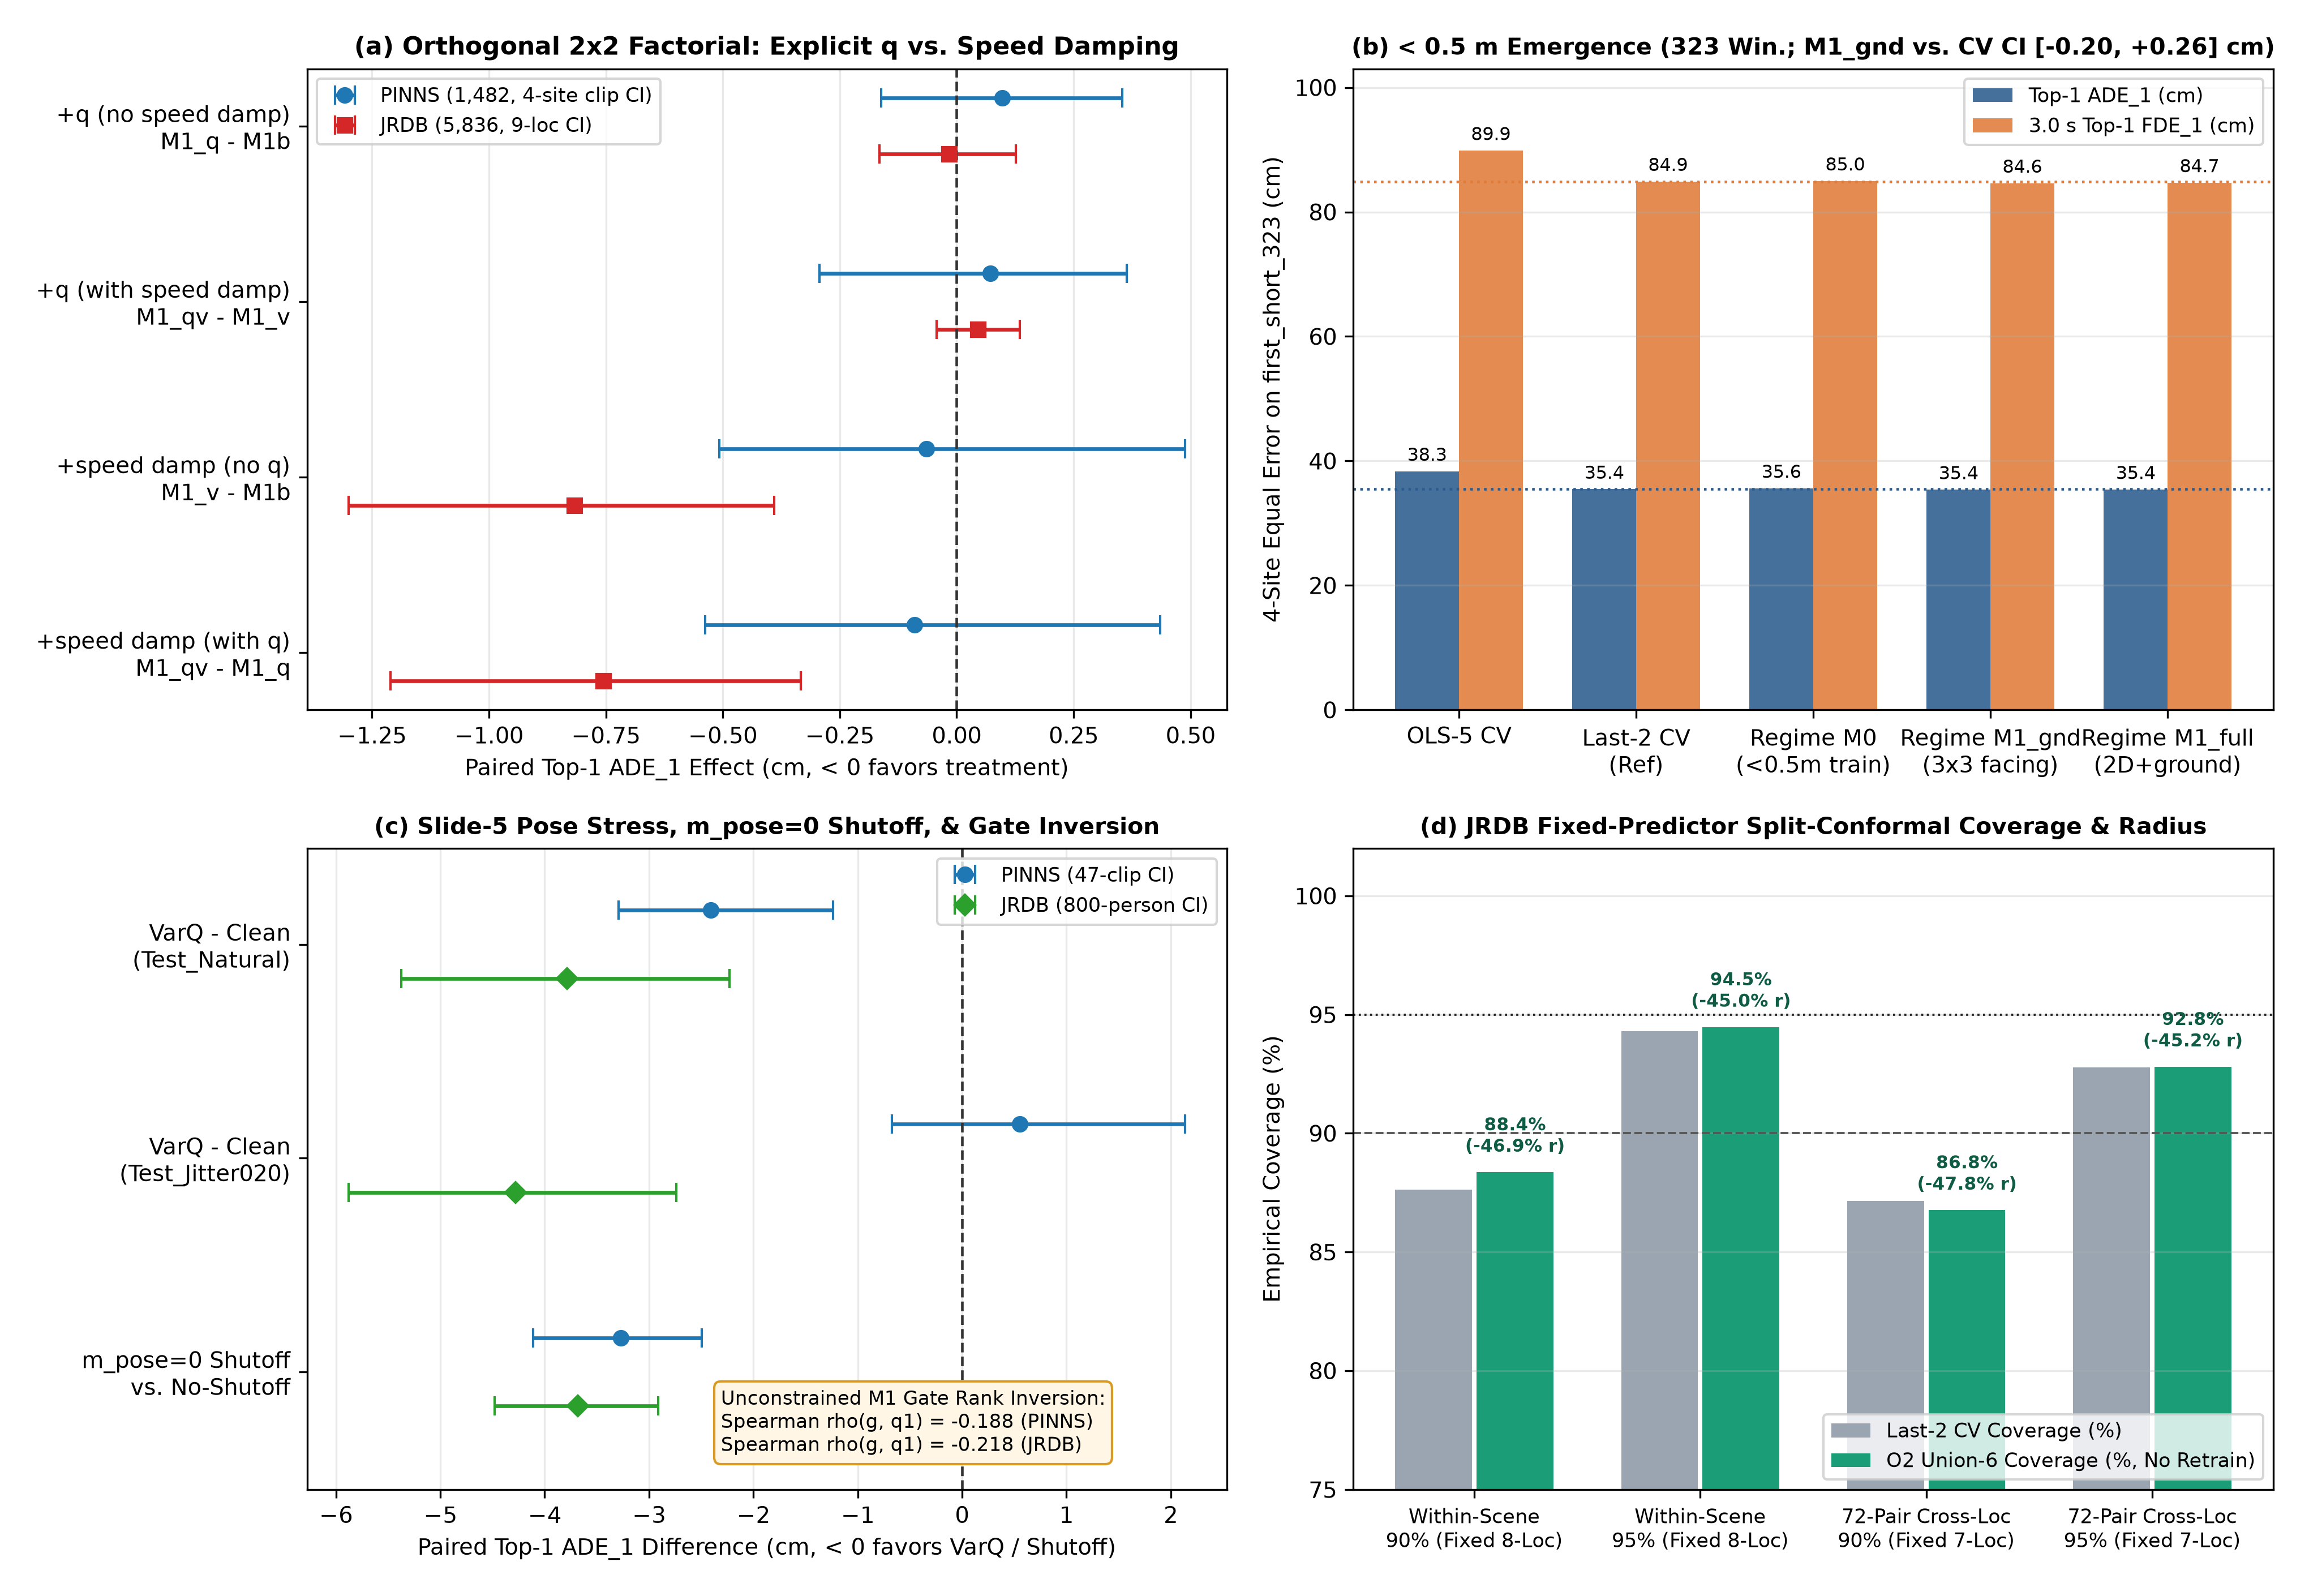
\includegraphics[width=0.96\textwidth]{fig18_wave17_factorial_slide5_and_jrdb_conformal.png}
\caption{正交 $2\times 2$ 析因、$<0.5\text{ m}$ 专域边界、关键点退化门控审计与 \texttt{JRDB} 共形覆盖。}
\label{fig:thu_f18}
\end{figure}

\begin{figure}[!htbp]
\centering
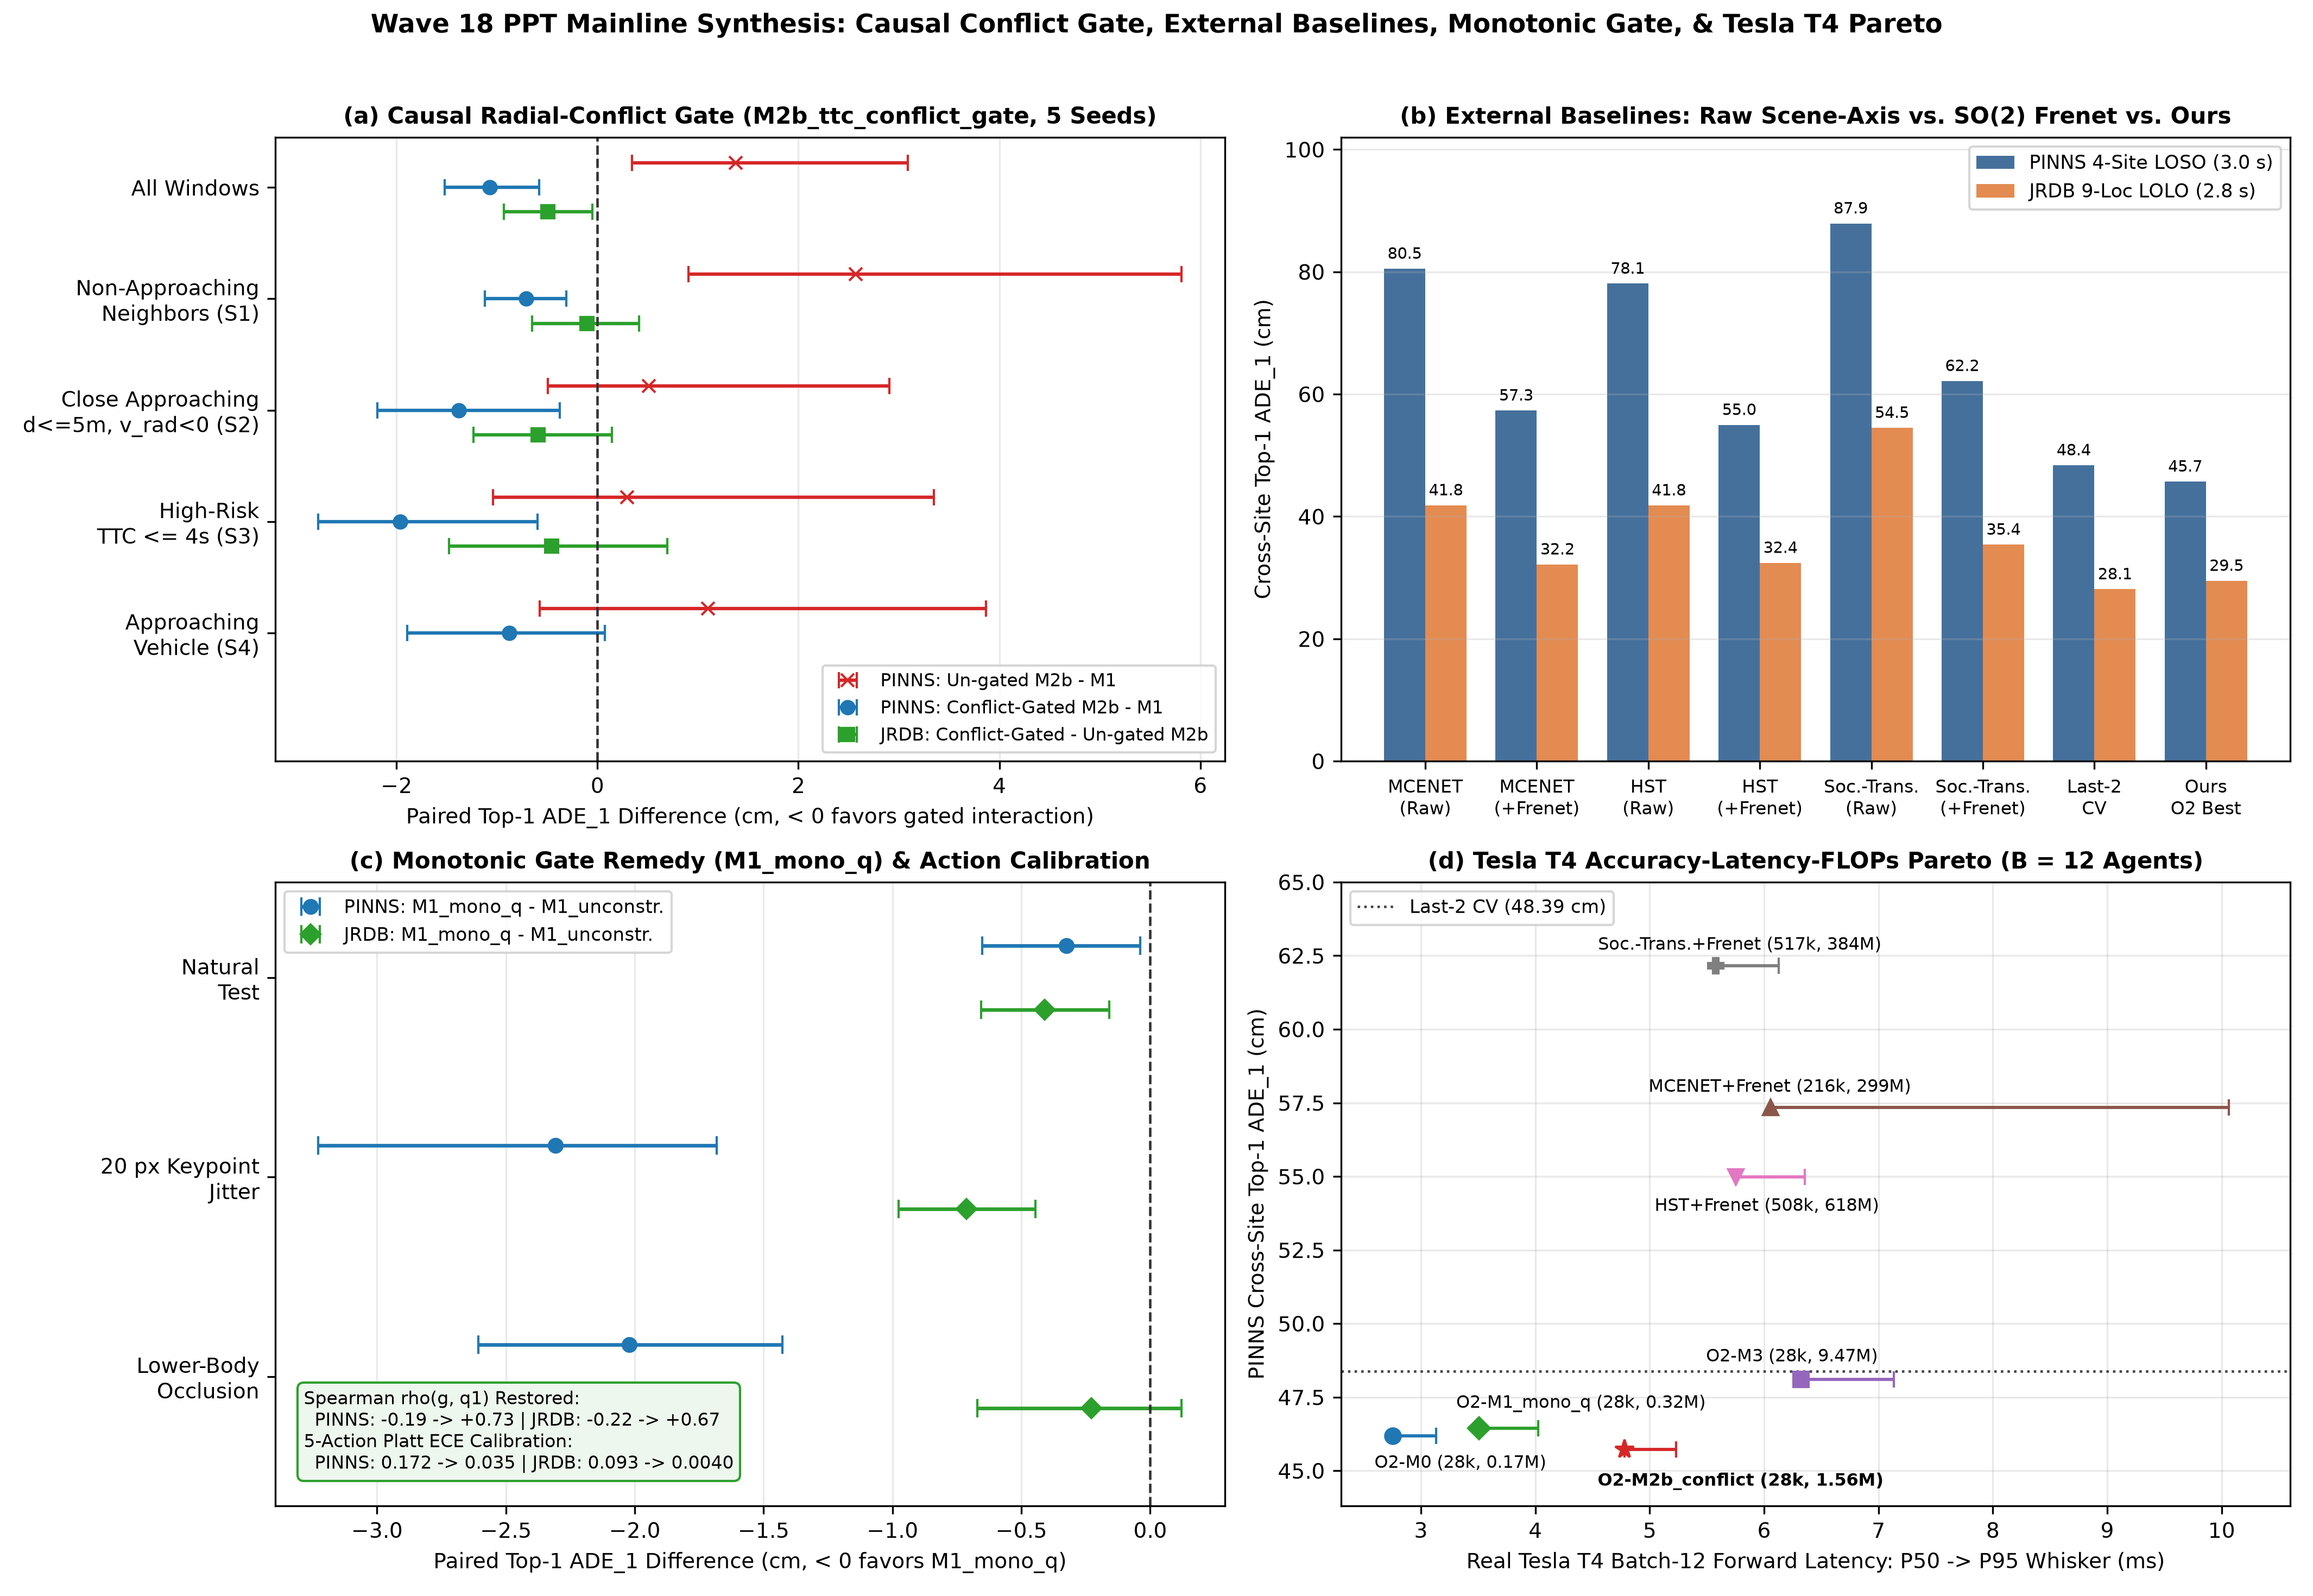
\includegraphics[width=0.96\textwidth]{fig19_wave18_conflict_rerank_ext_and_t4_pareto.png}
\caption{因果径向冲突门控、跨场景主流基线对比、结构单调门控修复与 \texttt{Tesla T4} 效率帕累托前沿。}
\label{fig:thu_f19}
\end{figure}

\begin{figure}[!htbp]
\centering
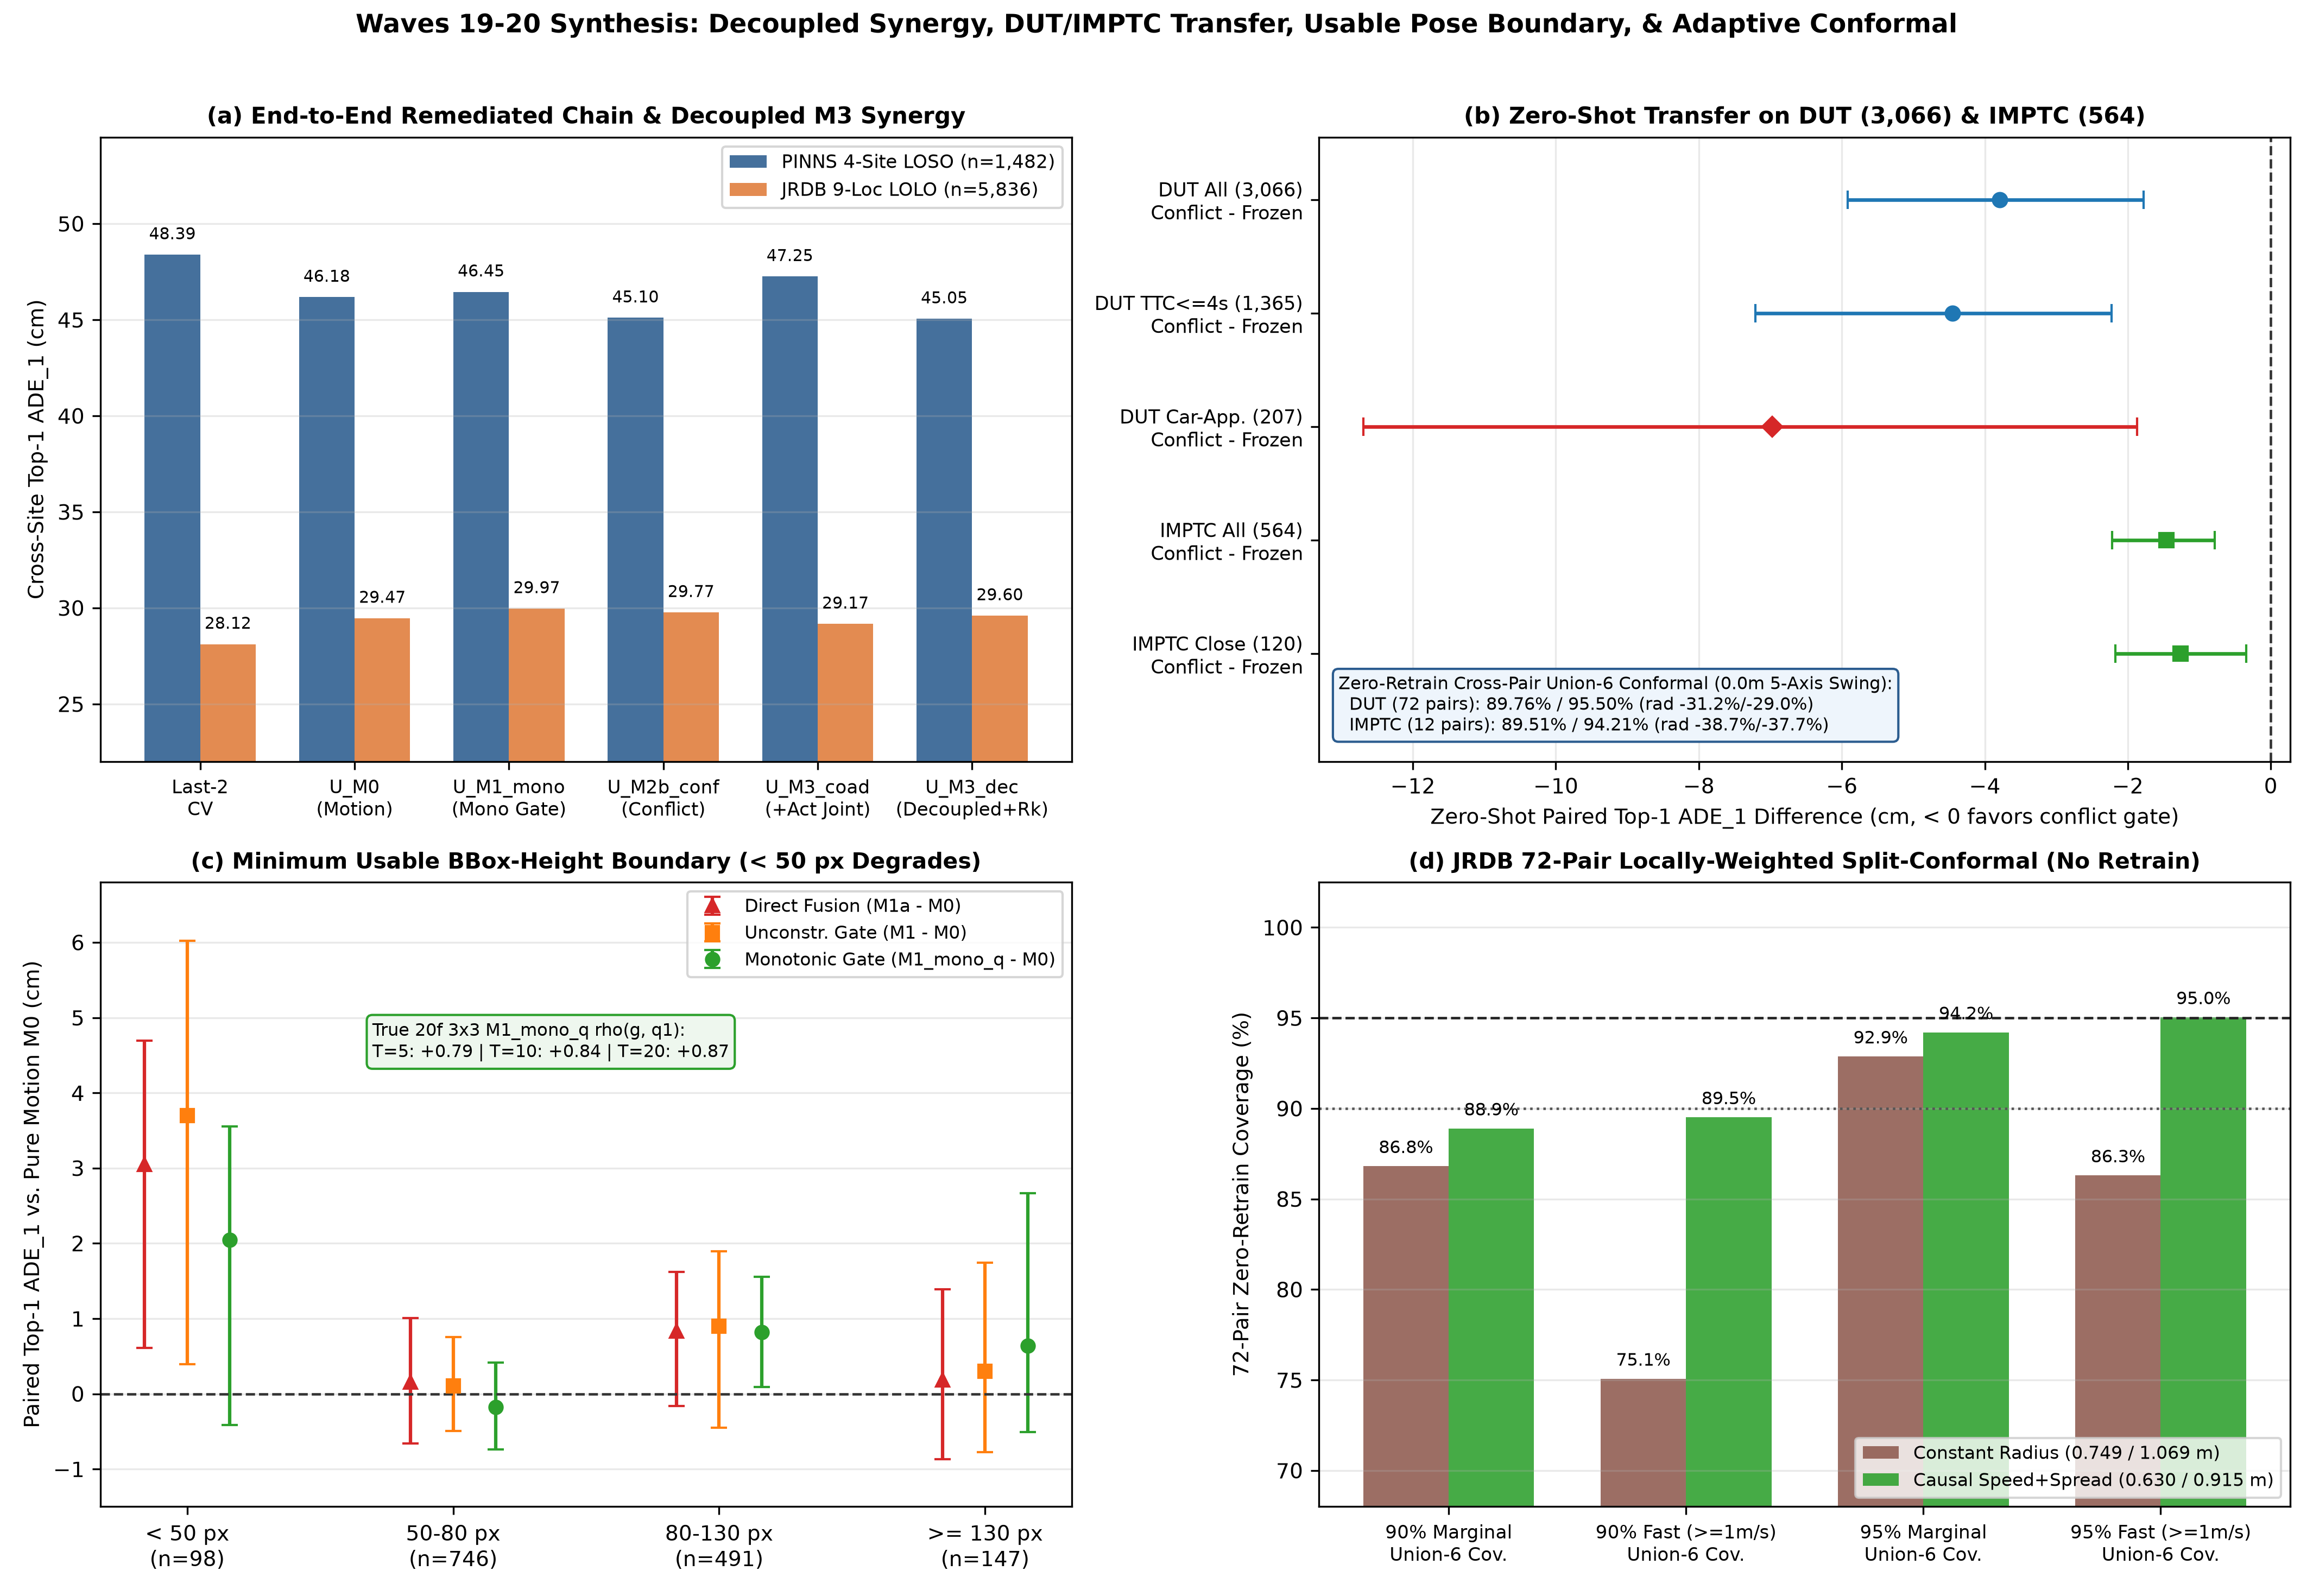
\includegraphics[width=0.96\textwidth]{fig20_wave19_20_unified_dut_boundary_and_adaptive_conformal.png}
\caption{解耦五动作协同、\texttt{DUT/IMPTC} 零样本迁移、最低可用像素框高边界与局部加权分裂共形。}
\label{fig:thu_f20}
\end{figure}

\section{零默认原视频初现复核、核心 $<0.5\text{ m}$ 边界校准、单因素消融与重现后预警验证}
围绕“实体遮挡后刚初现且五帧位移不足半米时，自动人体姿态能否比纯位置更优”，如表~\ref{tab:thu_w21_22} 与图~\ref{fig:thu_f21}--\ref{fig:thu_f22} 所示：（1）剔除此前 $45$ 窗默认归为前景人遮挡的分支，对 $26$ 段 \texttt{ori\_*.mp4} 中全部 $241$ 个非首帧窗口实施零默认逐窗复核（预注册哈希 \texttt{a2a869ed}），确证 $118/449$（$26.3\%$）个实体遮挡初现（车后 $32\ [\text{US }30, \text{IT }1, \text{TH }1]$、柱体/电杆/门洞 $66\ [\text{US }43, \text{JP }23]$、前景人 $20\ [\text{US }20]$；旧 $34$ 例 BEV 车后窗仅 $1/34$ 满足相机单应规则、$3/34$ 满足目视车后标签）及 $208$ 个首帧伪影。在\textbf{最贴近开题设定的 $<0.5\text{ m}$ 实体遮挡初现核心子组}（显式复核 $74$ 窗 / Wave-24 口径 $86$ 窗，均仅含 $1$ 次 \texttt{Start}）上，\textbf{无参数末两点匀速按窗口等权池化仍居最优}（$74$ 窗 $0.5249 / 1.1011\text{ m}$ vs.\ \texttt{CondMedoid} $0.5352\text{ m}$ $[+1.03\text{ cm}]$；$86$ 窗池化 $0.5453$ vs.\ $0.5527\text{ m}$，四地等权 $0.3578$ vs.\ $0.3808\text{ m}$）；逐站拆解证实此前四地等权下纯姿态跳升 $+4.02\text{ cm}$ 源于 \texttt{IT} ($N=1$) 与 \texttt{TH} ($N=1$) 合占 $50\%$ 站点权重且发生静止姿态漂移（池化 \texttt{S6\_M1} $-$ \texttt{S6\_M0} 仅 $+0.27\text{ cm}$ 跨零；静止安全门控 \texttt{ES6\_Full} 在四地等权达 $0.3528\text{ m}$ 追平匀速，池化仍高 $+2.12\text{ cm}$）。全集 $1{,}482$ 窗上 \texttt{S6\_Full\_CondMedoid} 达 $0.4382 / 0.9778\text{ m}$（CPU；\texttt{Tesla T4} 五种子 $0.4364 / 0.9709\text{ m}$），单因素消融证实 \texttt{+DelayedAPA}（池化 $-0.43\text{ cm}$）、\texttt{+CondScorer}（$-0.19/-0.21\text{ cm}$）与叠加 \texttt{Medoid}（$-0.73/-0.63\text{ cm}$）各自有效；无姿态冲突交互 \texttt{S6\_M2b} $-$ \texttt{S6\_M0} 在 $118$ 窗显著降 $-1.44 / -2.73\text{ cm}$，共视掩码姿态 \texttt{ES6\_M1} $-$ \texttt{S6\_M0} 在 $61$ 个显式初现机动窗降 $3.0\text{ s}$ 误差 $-0.96 / -1.69\text{ cm}$、起点后 $+0.5\text{ s}$ 降 $-1.13 / -1.81\text{ cm}$（衡量动作发生后的轨迹精度而非起点前报警时间）。\texttt{JRDB} 九地最低 $\text{ADE}_1$ 为无姿态 \texttt{S6\_M2b} $0.2772 / 0.5357\text{ m}$（\texttt{S6\_Full} $0.2786$，\texttt{CondMedoid} $0.2803 / 0.5422\text{ m}$）；\texttt{JTA-228} 输入为 $2$ 帧（$2.5\text{ Hz}$）二维屏幕关节（$0.90$ 固定置信度）+ 片段初 $\le 25$ 帧地面雅可比（$0.5564 / 1.1214\text{ m}$）。（2）在 \texttt{JAAD 2.0}~\cite{kotseruba2017jaad}（锁定测试 $953$ 窗：\texttt{Auto+Veh} $0.4888 / 1.1663$、\texttt{Human+Veh} $0.4910 / 1.1682$ vs.\ 匀速 $0.5003 / 1.1887$；$0.4250$ 实为 Wave 21 在广义 $406$ 窗数值；严格 $168$ 窗上单加自动姿态 $0.5039$ vs.\ 纯框 $0.5075$ 区间 $[-0.0097, +0.0058]$ 跨零，AP 升至 $0.8998 / 0.1640 / 0.5540$）上，核定测试负例分母为 $22/431 = 5.10\%$（验证集 $5\%$ 定阈漂移为纯框 $12/431=2.78\%$ vs.\ 自动姿态 $34/431=7.89\%$）：匹配 $22/431=5.10\%$ 后，自动 \texttt{RTMPose-17} 将 $12$ 次严格起步召回由 $2/12$ 升至 $6/12$（$+4$ 新命中、$0$ 丢失，双侧精确 McNemar $p=0.125$）、停步由 $0/10$ 升至 $3/10$；逐事件 $[f_{\text{last\_occ}}, f_{\text{reappear}}, f_{\text{alarm}}, f_{\text{onset}}]$ 核查证实 \textbf{$3/4$ 新增起步命中严格发生在完全恢复无遮挡（$t_{\text{alarm}}\ge t_{\text{reappear}}$）之后}（纯重现后可见帧协议下起步 $1/12\to 4/12$、停步 $0/10\to 3/10$）；共同命中在严格起步上 \texttt{AutoPose vs.\ KinOnly} 为 $n=2$（$0.0\text{ ms}$）、\texttt{AutoPose+Veh vs.\ VehOnly}（$n=5$）早报 $+340.0\text{ ms}$，全测试集起步（$n=10$）与横穿（$n=14$）早报 $+250.0 / +500.0\text{ ms}$。（3）双自动规则折线过滤（$\kappa_{\text{rule}}=0.8731$）穿线率 $0.27\%$，仍逊于 \texttt{No\_Map}（$0.4919\text{ m}$）。

\begin{table}[!htbp]
\centering
\caption{分区七大基准验证：四项含姿态基准与三项零姿态对照基准（五随机种子，统一单位与 $22/431=5.10\%$ 测试误报率）}
\label{tab:thu_w21_22}
\footnotesize
\begin{tabular}{llll}
\toprule
基准与物理单位 & 评测/核心初现规模 & 首选 $\text{ADE}_1/\text{FDE}_1$（匀速参照） & 核心边界与重现后同误报率审计 \\
\midrule
\multicolumn{4}{l}{\textit{A 组：含姿态基准（自动 2D/3D 视频骨架、2D+初帧雅可比或人工属性）}} \\
\texttt{PINNS}（m） & $1{,}482$ / 核心 $<0.5$m $74$ ($86$) & 全集 \textbf{0.4382} (T4 \textbf{0.4364})；$<0.5$m 池化 CV \textbf{0.5249} & $<0.5$m 池化 CV 最优；$118$ 窗 \texttt{M2b-M0} \textbf{$-2.73\text{ cm}$} \\
\texttt{JAAD 2.0}（框高） & 测试 $953$ / 严格解遮挡 $168$ & 测试 \texttt{Auto+V} \textbf{0.4888} / \texttt{Hum+V} 0.4910（CV 0.5003） & $22/431$ 下起步 $2/12\to\textbf{6/12}$ ($p{=}0.125$, \textbf{3/4 重现后}) \\
\texttt{JRDB}（m） & $5{,}836$ / 解遮挡 $507$ & \texttt{M2b} \textbf{0.2772}；\texttt{Full} 0.2786；\texttt{CondMed} 0.2803 & 最低 $\text{ADE}_1$ 为无姿态 \texttt{M2b}；机动 90 降 \textbf{$-1.18\text{ cm}$} \\
\texttt{JTA-228}*（m） & 锁定测试 $1{,}267$（2D+雅可比） & \texttt{M1} \textbf{0.5564 / 1.1214}（\texttt{M0} 0.5602, CV 0.5659） & $2$ 帧 2D 屏幕关节+初帧雅可比降 \textbf{$-0.38\text{ cm}$} \\
\midrule
\multicolumn{4}{l}{\textit{B 组：零姿态运动与交互对照基准（全程 $m_{\text{pose}}\equiv 0$ 严格校验）}} \\
\texttt{ETH/UCY}~\cite{pellegrini2009eth}（m） & 五场景 $4{,}187$（无姿态） & \texttt{Full} 0.3919 $>$ CV \textbf{0.3892}（$+0.27\text{ cm}$） & 主动机动窗降 \textbf{$-9.11 / -11.08\text{ cm}$}；零姿态泄漏 $0.0\text{ cm}$ \\
\texttt{DUT + IMPTC}（m） & $3{,}066$（$<0.5$m $400$）+ $564$（$365$） & \texttt{DUT} \textbf{0.3483}（CV 0.5067）；\texttt{IMPTC} \textbf{0.2061} & \texttt{IMPTC} $<0.5$m：0.2126$\to$\textbf{0.1942}/0.2004；零样本摆动 $0.0\text{ m}$ \\
\bottomrule
\end{tabular}
\end{table}

\begin{figure}[!htbp]
\centering
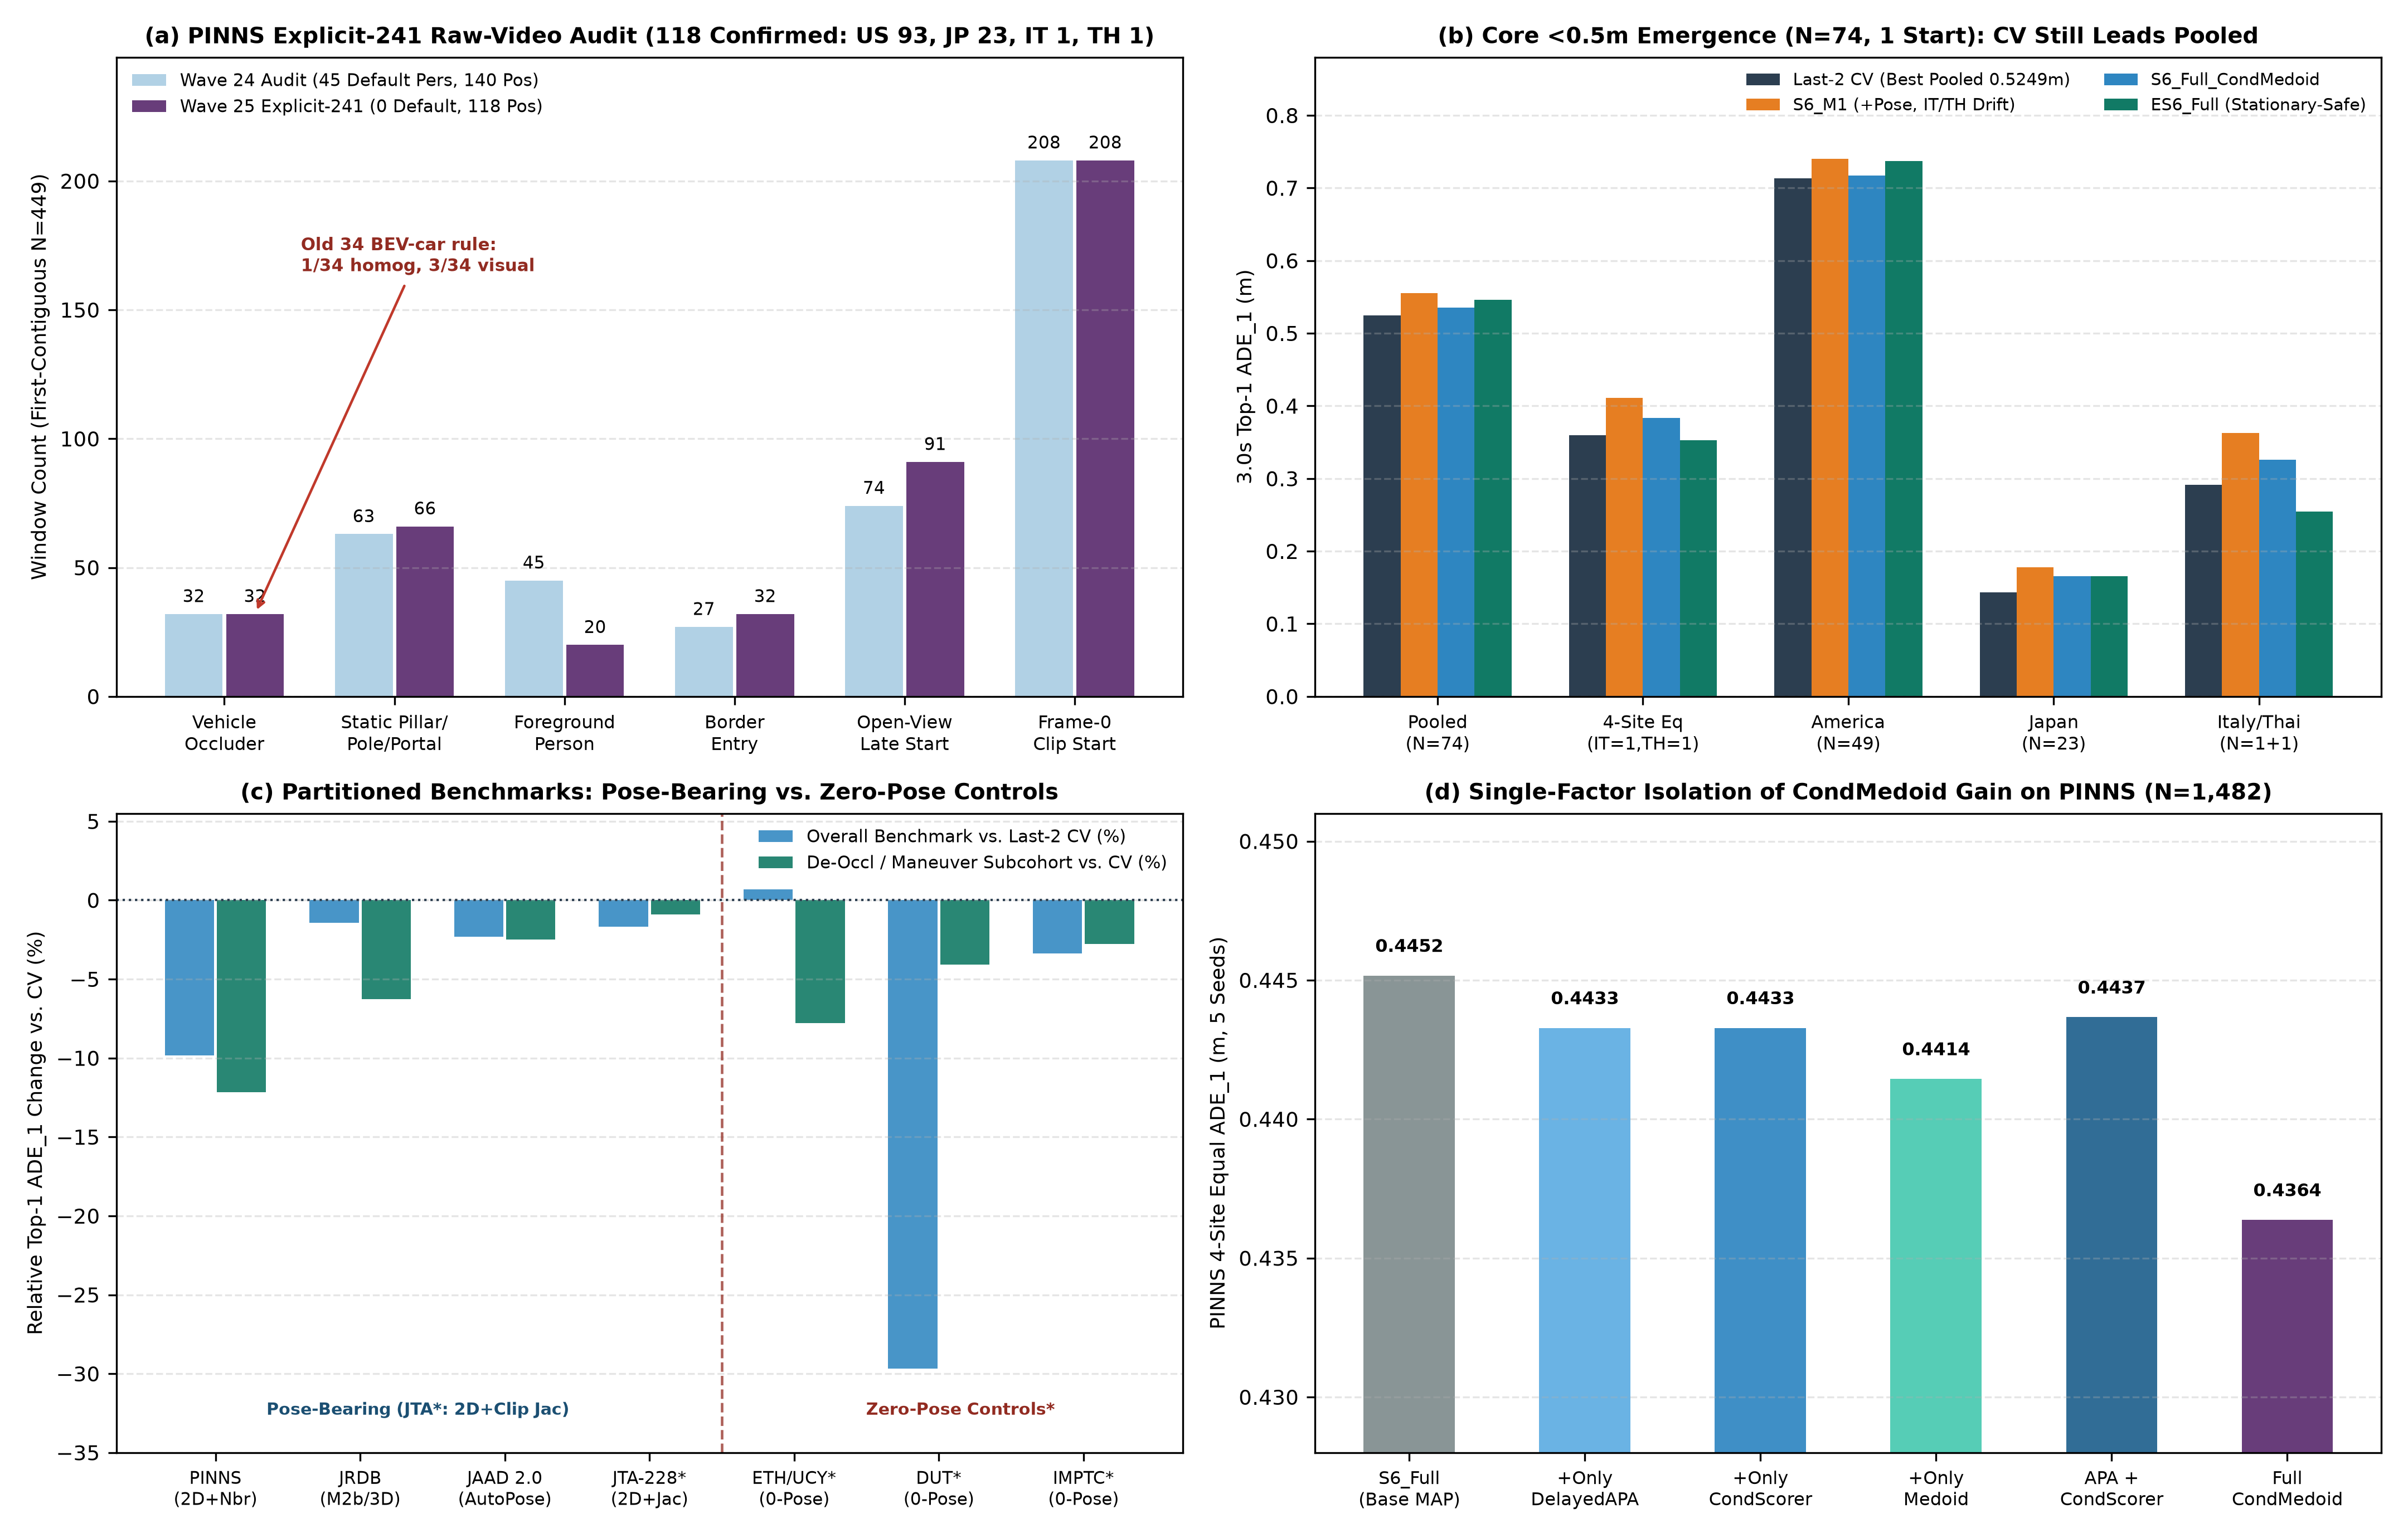
\includegraphics[width=0.96\textwidth]{fig21_wave21_true_emergence_6slot_and_7dataset_precursors.png}
\caption{\texttt{PINNS} 零默认 $241$ 窗原视频初现复核（确认实体遮挡 $118$ 窗、首帧伪影 $208$ 窗）、核心 $<0.5\text{ m}$ 初现（$N=74$）池化与逐站拆解（匀速池化最优 $0.5249\text{ m}$）、分区七基准对比及 \texttt{CondMedoid} 单因素消融。}
\label{fig:thu_f21}
\end{figure}

\begin{figure}[!htbp]
\centering
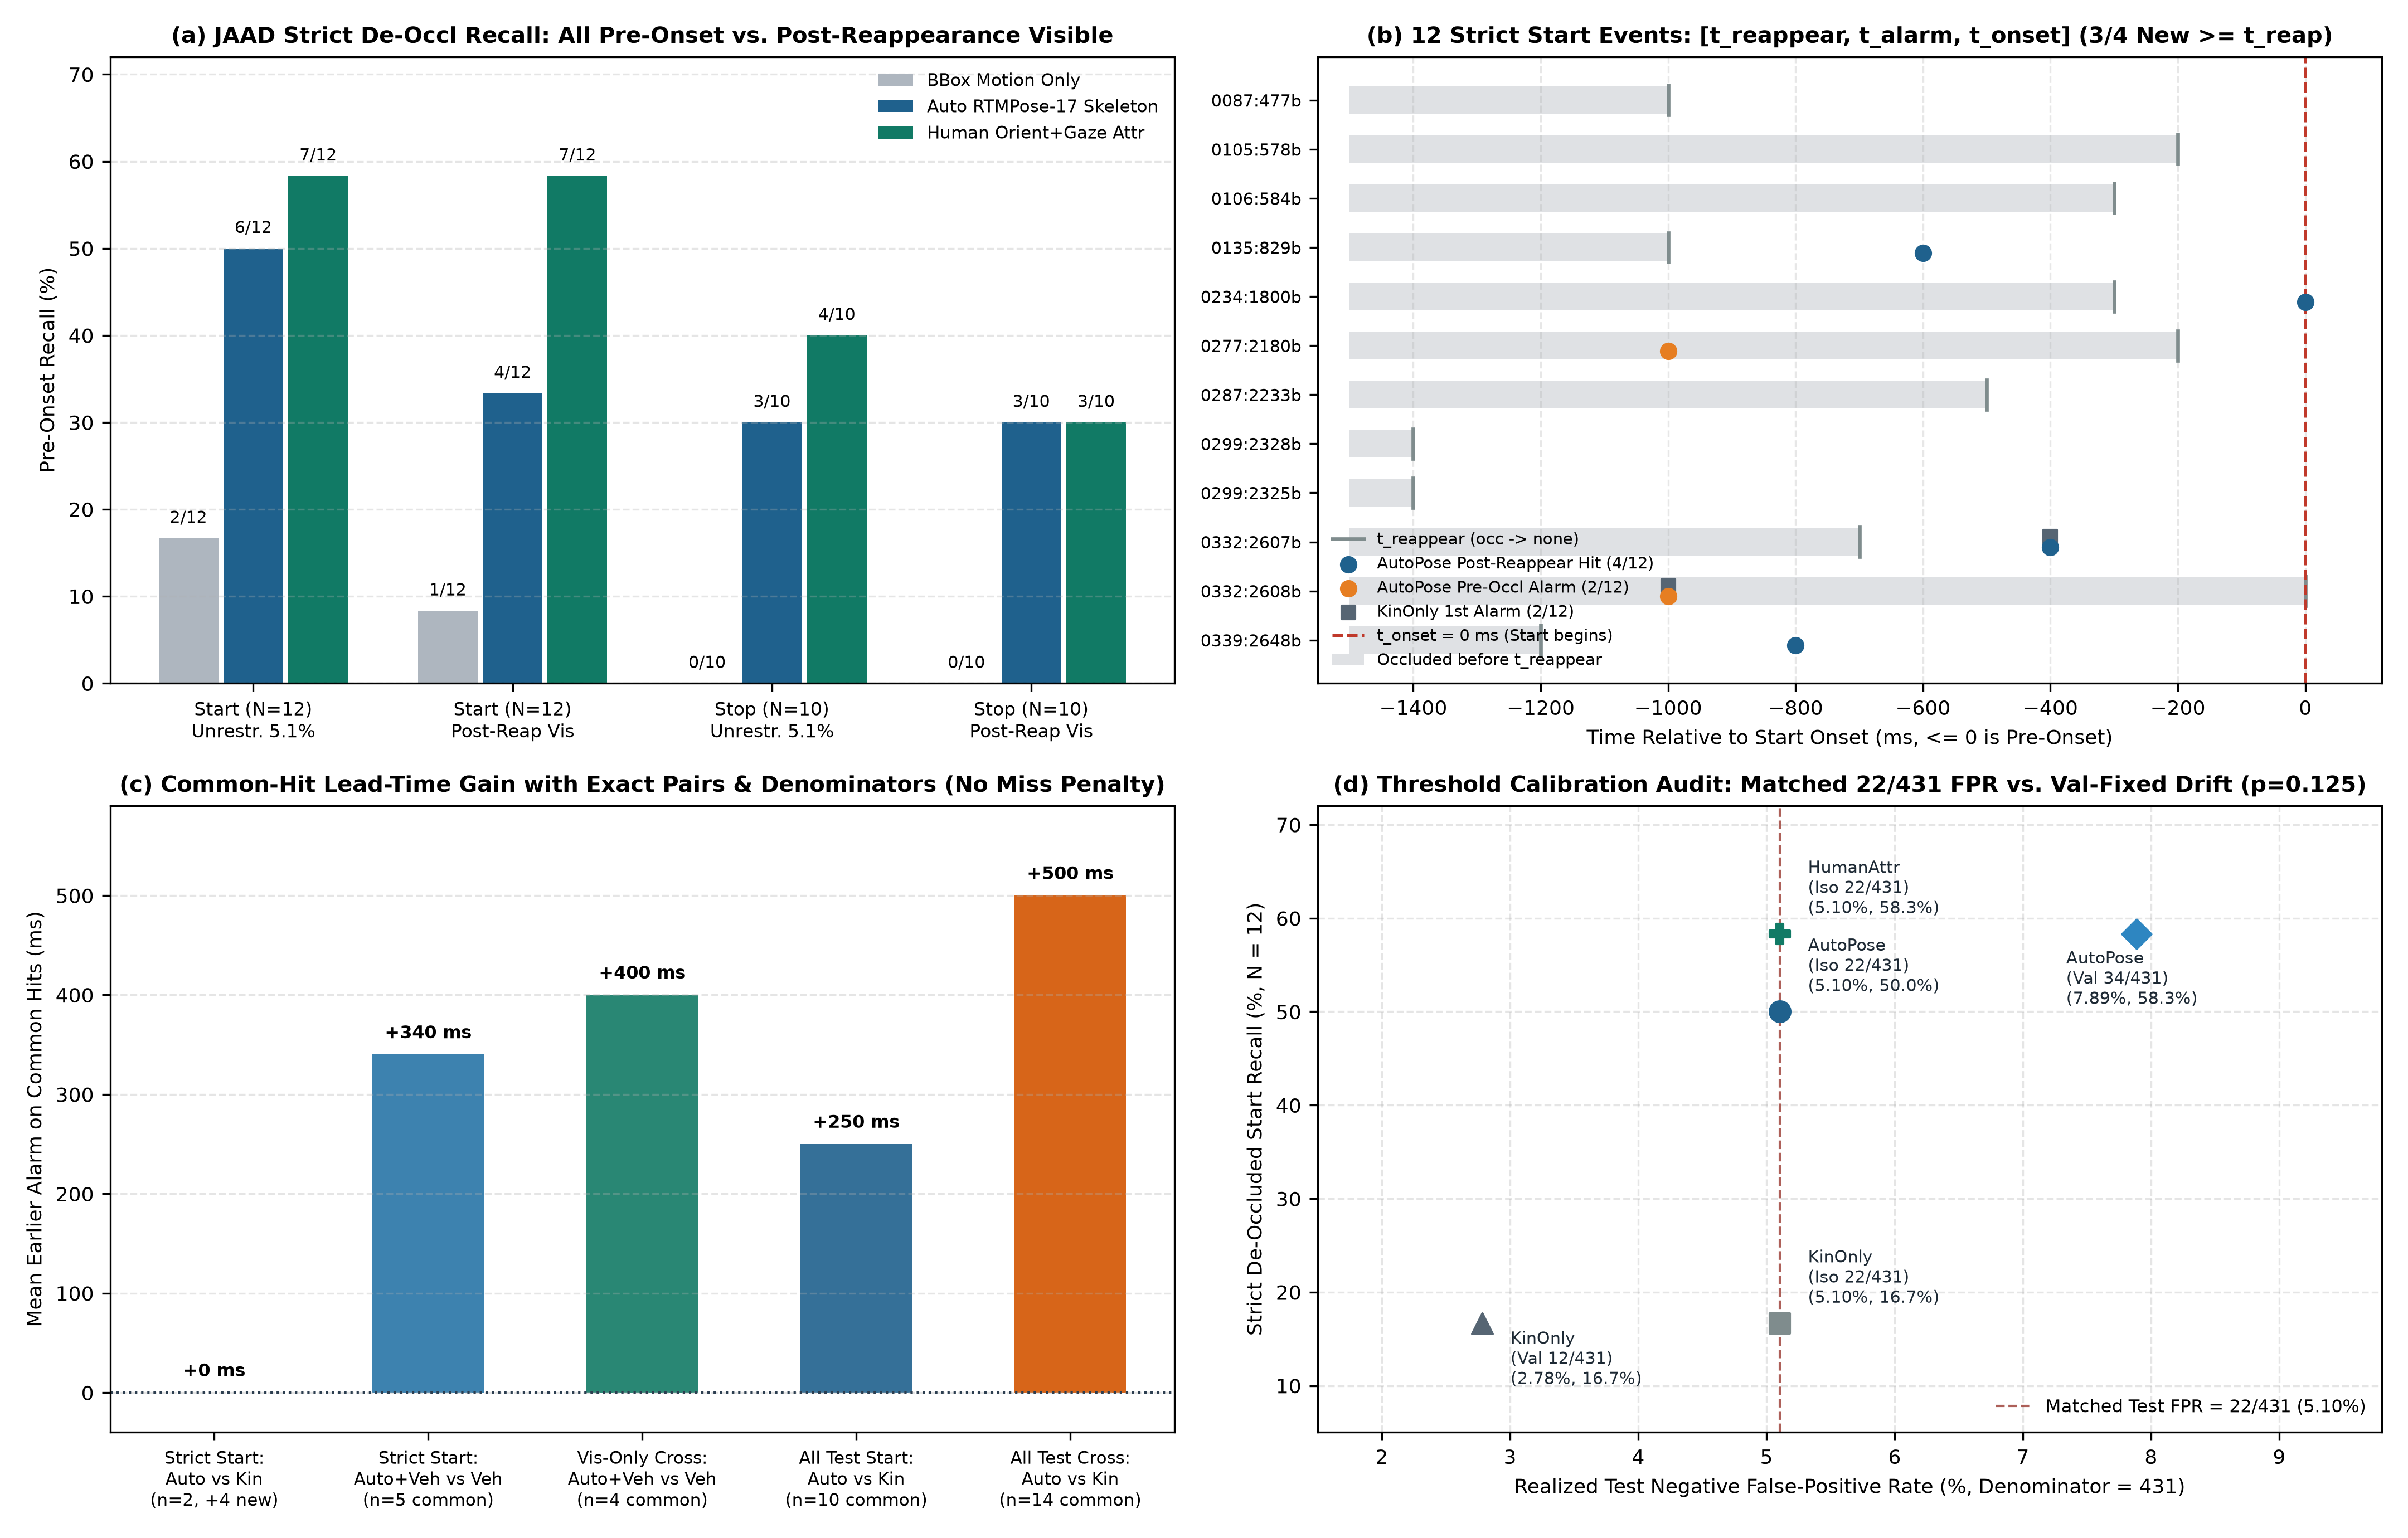
\includegraphics[width=0.96\textwidth]{fig22_wave22_apa_leadtime_and_delayed_onset.png}
\caption{\texttt{JAAD 2.0} 严格解遮挡召回（全窗口 vs.\ 重现后可见帧）、$12$ 次起步 $[t_{\text{reappear}}, t_{\text{alarm}}, t_{\text{onset}}]$ 逐事件时序（$3/4$ 新命中 $\ge t_{\text{reappear}}$）、共同命中精确分母及 $22/431$ 匹配误报率 vs.\ 验证集定阈漂移（$p=0.125$）。}
\label{fig:thu_f22}
\end{figure}

\chapter{讨论与局限性分析}
（1）\textbf{核心 $<0.5\text{ m}$ 实体遮挡初现与小样本报警边界：}即便完成零默认原视频复核（$118/449$ 实体遮挡初现）与静止安全门控（\texttt{ES6\_Full}），在\textbf{最贴近开题设定的 $<0.5\text{ m}$ 实体遮挡初现核心子组（显式 $74$ 窗 / Wave-24 $86$ 窗，仅含 $1$ 次 \texttt{Start}）上，无参数末两点匀速按窗口池化仍居最低误差（$0.5249 / 1.1011\text{ m}$ 与 $0.5453 / 1.1322\text{ m}$）}（\texttt{ES6\_Full} 消除 \texttt{IT=1/TH=1} 静止漂移后在四地等权达 $0.3528\text{ m}$ 追平匀速，池化仍高 $+2.12\text{ cm}$）；车载平视（\texttt{JAAD 2.0}）在匹配 $22/431=5.10\%$ 测试误报率下将起步召回由 $2/12$ 升至 $6/12$（$p=0.125$，$3/4$ 新命中严格在 $t_{\text{reappear}}$ 后触发，纯可见帧 $1/12\to 4/12$），但独立 $2.0\text{ s}$ 轨迹收益跨零且受限于小事件分母（$N=12$）；框高 $<50\text{ px}$ 或 $q_1 < 0.75$ 须依赖单调门控压低权重。（2）\textbf{静态折线边界：}双自动几何与因果轨迹规则过滤（$\kappa_{\text{rule}}=0.8731$，穿线率 $0.27\%$）仍逊于 \texttt{No\_Map}（$0.4919\text{ m}$）。（3）\textbf{全部可复现资产：}全部 64 份云端结果归档均通过双层 SHA-256 核验并开源复现代码（\url{https://github.com/pjyyyds/Unstructured-ShortPose-Pred}）。

\chapter{总结与展望}
本文针对非结构化道路短时可变质量姿态下的行人动作与轨迹联合预测，提出了正交奇偶等变 Frenet 规范化、结构单调质量门控、因果径向冲突门控（$118$ 窗 \texttt{M2b-M0} 降 $-1.44/-2.73\text{ cm}$，\texttt{JRDB} 最低 $\text{ADE}_1 = 0.2772\text{ m}$）、解耦五动作校准重排、经单因素验证的条件化六槽中位解码（\texttt{PINNS} 全集达 $0.4382 / 0.9778\text{ m}$、\texttt{Tesla T4} $0.4364 / 0.9709\text{ m}$，$61$ 个显式初现机动窗 \texttt{ES6\_M1-M0} 降 $-0.96/-1.69\text{ cm}$；同时诚实确立 $<0.5\text{ m}$ 实体初现核心子组池化仍由匀速 $0.5249\text{ m}$ 领先）与源折局部加权零重训分裂共形方法，在四项含姿态基准与三项零姿态对照基准上实现了紧凑参数（$20.7\text{k}\text{--}28.0\text{k}$）、毫秒级延迟（\texttt{Tesla T4} $2.75\text{--}4.78\text{ ms}$）且正负结论透明可复核的预测体系。未来工作将进一步面向车载双目/激光深度融合与实车嵌入式闭环避障验证展开。

\bibliographystyle{IEEEtran}
\bibliography{references}

\end{document}
